\documentclass[conference,10pt]{IEEEtran}
\IEEEoverridecommandlockouts
\usepackage[T1]{fontenc}
\usepackage{graphicx,booktabs,amsmath,amssymb,multirow,xcolor,url,xspace}
\usepackage[hidelinks]{hyperref}
\hypersetup{pdftitle={Egocentric Human Demonstrations for a Bimanual Robot: Combined Report}, pdfauthor={Jeong Hwan Lee}}
\usepackage{tikz}
\usetikzlibrary{positioning,arrows.meta,fit,backgrounds}
\newcommand{\mm}{\,mm\xspace}
\newcommand{\cmt}[1]{}
\def\UrlBreaks{\do\/\do\_\do\.\do\-}\def\UrlFont{\small\ttfamily}\newcommand{\code}[1]{\path{#1}}
% Each part restarts its section numbering; hyperref anchors carry the part number so they stay unique.
\newcounter{rpart}
\renewcommand{\theHsection}{\arabic{rpart}.\arabic{section}}
\renewcommand{\theHsubsection}{\arabic{rpart}.\arabic{section}.\arabic{subsection}}
\newcommand{\reportpart}[3]{\clearpage\stepcounter{rpart}\setcounter{section}{0}%
  \twocolumn[{\centering{\LARGE\bfseries #1\par}\vspace{1.5mm}{\large #2\par}\vspace{3mm}\hrule\vspace{5mm}}]\label{#3}}
\newcommand{\partabstract}[1]{\noindent\textbf{\textit{Abstract}}---\textit{#1}\par\medskip}

\begin{document}
\title{Egocentric Human Demonstrations for a Bimanual Robot\\[1mm]\Large Combined Report: Part I, Part II and Methods}
\author{\IEEEauthorblockN{Jeong Hwan Lee}
\IEEEauthorblockA{Technical report, version 4.1, 12 October 2026 \quad alnrg2arg@gmail.com\\
Code, results and sample data are available on request.}}
\maketitle
\begin{abstract}
The capture device, HandUMI, is an open-source design by BrikHMP18 (murobotics-ai/handumi-hw), not our design.
This document combines the three reports of version 4.1 into one file, unchanged in content: Part I (full length) on 349
bimanual egocentric HandUMI demonstrations of three-cube stacking, the capture hardware, the processing funnel, X-VLA
training, offline evaluation and transfer to the reBot B601; Part II (full length) on single-arm approach data, object-based
scale, robot-side calibration, a shared task frame and deployment settings; and the Methods document, which describes how
every stage of the pipeline works rather than its results. Each part keeps its own abstract, section numbering and
figures; references such as ``Part I, Sec.~III'' refer to the section numbers printed in that part. The bibliography of the
three parts is merged at the end.
\end{abstract}

\noindent\textbf{Contents.}
\begin{itemize}
\item Part I: Three-Cube Stacking \dotfill p.~\pageref{part:p1}
\item Part II: Single-Arm Approach to a Cube \dotfill p.~\pageref{part:p2}
\item Methods and Pipeline \dotfill p.~\pageref{part:m}
\item References \dotfill p.~\pageref{part:refs}
\end{itemize}

\reportpart{Part I}{Three-Cube Stacking (bimanual)}{part:p1}
\partabstract{We study how far natural egocentric human demonstrations, recorded with HandUMI, an open-source hand-worn UMI-style gripper designed and published by BrikHMP18 (not our design), can be turned into
training data for a bimanual robot policy. We collected 349 bimanual demonstrations of a three-cube stacking task with six
stacking orders balanced at collection time (51--64 episodes per order), using per-hand wrist fisheye cameras, IMUs and jaw
encoders plus a fixed head camera. A multi-stage pipeline (MASt3R-SLAM wrist poses with per-episode visual--inertial scale,
retargeting to a 6-DoF robot arm, and synchronisation, workspace, metric and inverse-kinematics gates) keeps 259 episodes, or
561 bimanual 65-frame segments. On these we fine-tune a 0.9B-parameter vision-language-action model (X-VLA) to predict 30-step
joint-space action chunks, and evaluate it offline on 26 held-out episodes. The median held-out TCP error is 1.5--5.7\mm over a
0.2--1.2\,s horizon. This figure is dominated by static phases: on the 23\% of samples in which the target moves at least
20\mm, the error at 1.2\,s is 39.9\mm, direction cosine 0.90, and the policy reduces joint error by 24\% relative to a
zero-motion predictor. Swapping the order instruction changes the predicted motion measurably but by only ${\sim}8\%$ of its
magnitude, and the true instruction predicts the human motion no better than the five wrong ones, so the model makes no
task-useful use of the order instruction in this evaluation.
Two follow-ups address the main bottleneck. Replacing the single-anchor retarget with multi-seed trajectory-window
retrieval raises the usable fraction of candidate segments from 36.5\% to 56.1\% and brings the retargeted postures
much closer to real robot postures; a 60-episode robot-like re-collection is used to test whether collection style changes
retarget feasibility; it does not appreciably, a negative, diagnostic result. Fine-tuned on 150 robot demonstrations, the ego-pretrained model has a
10\% lower geo score than an otherwise identical model trained from scratch (95\% CI 5.6--14.7\%), but only on episodes
contained in both training sets.
This version adds a third stage that removes joint-space retargeting altogether. Whole human episodes are converted to
relative Cartesian end-effector actions in the same 20-dimensional layout as our robot data, with no workspace or IK
filtering (330 episodes, 48{,}411 training rows after a pose-jump filter). An audit of the public X-VLA base shows that only 8
of its 30 domain soft-prompt slots were ever trained, which changes how earlier runs should be read. On robot camera frames the
ego-only model predicts no useful motion direction (median cosine $-0.05$/$-0.03$ versus $+0.81$/$+0.77$ for a robot-trained
model); swapping images and states between domains locates the gap in the wrist images, whose sharpness differs by about
30$\times$. Used as an initialization for robot fine-tuning, the ego model starts at a 3.9$\times$ lower training loss, but the advantage
shrinks to a tie by 60k steps of an otherwise identical run. Version 4 adds a low-data ablation: three otherwise identical
fine-tuning runs on only 30 robot episodes, from the base model and from ego pretraining checkpoints at 100k and 300k steps.
Both ego initializations start at less than half the scratch training loss; the advantage is gone by about 100k steps
(100k-step pretraining) and about 200k steps (300k-step pretraining), and all three runs overfit 30 episodes heavily. None of
them has yet been run on the robot. An ego-initialized model fine-tuned on 312 robot episodes completed full three-cube
stacks in closed loop, but trials were not counted, so we report a demonstration, not a success rate. No experiment tests
new spatial layouts or unseen stacking orders; we state explicitly which claims this data can and cannot support. The
single-arm approach work that was Sec.~XII of version 3 now forms Part II. Version 4.1 adds a description of the capture
hardware: the upstream HandUMI design we built, the parts we changed, and the IMU we added.}
\section{Introduction}\label{p1:sec:intro}
Collecting robot demonstrations is often expensive, requiring access to a physical robot, an operator and task-specific
teleoperation infrastructure. Egocentric human
demonstrations can be collected faster, with less hardware, in natural settings, and hand-worn grippers such as UMI~\cite{chi2024umi}
make the human's end-effector look like the robot's, reducing the embodiment gap at the gripper. Whether such data
transfers to a specific robot depends on a chain of steps that is rarely audited end to end: sensor calibration, metric pose
recovery from a moving wrist camera, retargeting into the robot's kinematics, and the filtering that decides which human motion
is kept at all. Each step can silently change what a policy ends up learning.

This report documents one complete pass through that chain on real data and asks a deliberately narrow question:
\emph{after all processing, how much robot-executable action structure does a pretrained vision-language-action (VLA) model
learn from retargeted egocentric human demonstrations, and does it use the task-order instruction?} Our contributions are:
\begin{itemize}
\item a build record of the hand-worn capture hardware: the upstream design, three modified parts, an added wrist IMU
with its firmware protocol, and the device-identity pitfalls (Sec.~\ref{p1:sec:hw});
\item a 349-episode bimanual egocentric dataset of three-cube stacking with six balanced stacking orders, with full sensor
calibration and per-episode metadata (Sec.~\ref{p1:sec:data});
\item a documented processing funnel from raw human video to robot joint-space segments, reporting what each gate removes
(Sec.~\ref{p1:sec:proc});
\item an offline evaluation of a 0.9B-parameter VLA fine-tuned on the result, including a motion-gated analysis showing that
aggregate errors are dominated by static phases, and a prompt-swap test of instruction use (Secs.~\ref{p1:sec:eval}--\ref{p1:sec:fail});
\item follow-up experiments on the retargeting bottleneck, robot-like re-collection and ego-to-robot fine-tuning (Sec.~\ref{p1:sec:follow});
\item a Cartesian conversion of whole episodes that matches the robot's action contract, with the pose-jump failure it
exposed (Sec.~\ref{p1:sec:v3}), and transfer diagnostics that separate visual, state and initialization effects (Sec.~\ref{p1:sec:transfer});
\item a low-data ablation of ego pretraining length on 30 robot episodes (Sec.~\ref{p1:sec:r30}).
\end{itemize}
We are explicit about scope. The evaluation is open-loop on held-out \emph{episodes}; it is not a closed-loop robot test,
and because layouts were not recorded and all six orders appear in training, it measures neither spatial nor task-order
generalization. Sections~\ref{p1:sec:intro}--\ref{p1:sec:follow} are unchanged in substance from version 2 (30 September 2026) and
Sections~\ref{p1:sec:v3}--\ref{p1:sec:transfer} from version 3 (4 October 2026), apart from run status; Sec.~\ref{p1:sec:r30} is new in version 4 and Sec.~\ref{p1:sec:hw} in version 4.1 (12 October 2026).
Version 3 also contained a single-arm approach study; it has grown into a separate report (Part II), which reuses the
device, pose pipeline and action contract described here. Sec.~\ref{p1:sec:lim} lists the experiments needed for the claims we
do not make.

\section{Related and Motivating Work}
\textbf{Portable demonstration interfaces.} UMI~\cite{chi2024umi} records hand-held gripper demonstrations with a wrist fisheye
camera and recovers poses with ORB-SLAM3 against a per-scene map; DexCap~\cite{wang2024dexcap} and related systems target dexterous
hands. Our device is HandUMI~\cite{handumi_hw}, an open-source hand-worn UMI variant for parallel-jaw grippers with a
servo-encoder jaw. We replace its VR tracking with a wrist IMU and add a fixed head camera (Sec.~\ref{p1:sec:hw}).
\textbf{Learning from egocentric humans.} EgoMimic~\cite{kareer2024egomimic} and MimicPlay~\cite{wang2023mimicplay} co-train robot
policies on human egocentric video and robot data; large egocentric corpora such as Ego4D~\cite{grauman2022ego4d} motivate the
scaling argument. These works report closed-loop gains; we instead audit what survives processing and what a model learns
offline, which is a prerequisite for interpreting such gains.
\textbf{Policies.} Action-chunking imitation (ACT~\cite{zhao2023act}, Diffusion Policy~\cite{chi2023diffusion}) and VLA models
(OpenVLA~\cite{kim2024openvla}, $\pi_0$~\cite{black2024pi0}, X-VLA~\cite{zheng2025xvla}) predict multi-step action chunks from
images and language. We use X-VLA through LeRobot~\cite{cadene2024lerobot} because its flow-matching~\cite{lipman2023flow} head
and soft prompts accommodate a new embodiment with a small dataset.
\textbf{Pose recovery.} MASt3R-SLAM~\cite{murai2025mast3rslam} provides dense monocular SLAM from a 3D reconstruction prior; we
combine it with IMU-based scale estimation, calibrated with Kalibr~\cite{furgale2013kalibr}.

\begin{figure*}[t]
\centering
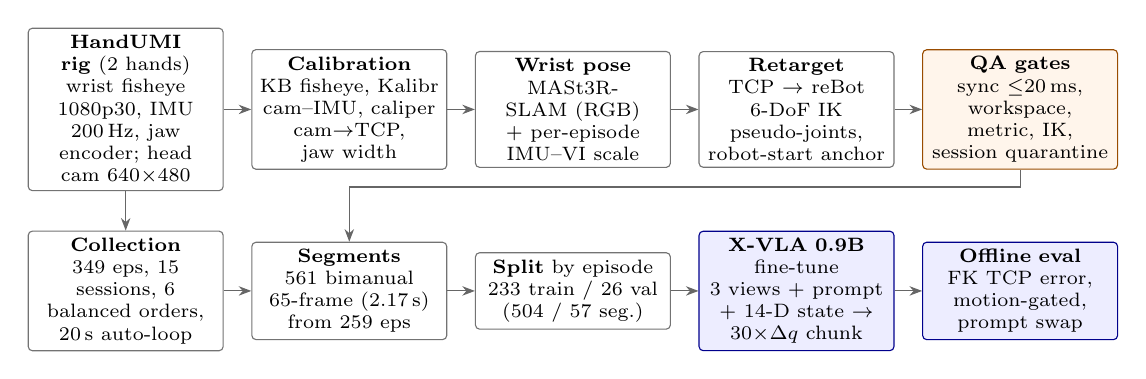
\begin{tikzpicture}[font=\scriptsize, node distance=3.5mm and 3.5mm,
  box/.style={draw=black!55, rounded corners=1.5pt, align=center, inner sep=2.5pt, minimum height=9.5mm, text width=23mm, fill=white},
  gate/.style={box, fill=orange!8, draw=orange!60!black},
  learn/.style={box, fill=blue!7, draw=blue!55!black},
  arr/.style={-{Stealth[length=1.6mm]}, draw=black!60}]
\node[box] (dev) {\textbf{HandUMI rig} (2 hands)\\wrist fisheye 1080p30, IMU 200\,Hz, jaw encoder; head cam 640$\times$480};
\node[box, right=of dev] (cal) {\textbf{Calibration}\\KB fisheye, Kalibr cam--IMU, caliper cam$\to$TCP, jaw width};
\node[box, right=of cal] (pose) {\textbf{Wrist pose}\\MASt3R-SLAM (RGB) + per-episode IMU--VI scale};
\node[box, right=of pose] (ret) {\textbf{Retarget}\\TCP $\to$ reBot 6-DoF IK pseudo-joints, robot-start anchor};
\node[gate, right=of ret] (qa) {\textbf{QA gates}\\sync $\le$20\,ms, workspace, metric, IK, session quarantine};
\node[box, below=5mm of dev] (col) {\textbf{Collection}\\349 eps, 15 sessions, 6 balanced orders, 20\,s auto-loop};
\node[box, right=of col] (seg) {\textbf{Segments}\\561 bimanual 65-frame (2.17\,s) from 259 eps};
\node[box, right=of seg] (split) {\textbf{Split} by episode\\233 train / 26 val (504 / 57 seg.)};
\node[learn, right=of split] (vla) {\textbf{X-VLA 0.9B} fine-tune\\3 views + prompt + 14-D state $\to$ 30$\times$$\Delta q$ chunk};
\node[learn, right=of vla] (ev) {\textbf{Offline eval}\\FK TCP error, motion-gated, prompt swap};
\draw[arr] (dev)--(cal); \draw[arr] (cal)--(pose); \draw[arr] (pose)--(ret); \draw[arr] (ret)--(qa);
\draw[arr] (dev)--(col); \draw[arr] (qa.south) |- ++(0,-2.2mm) -| (seg.north);
\draw[arr] (col)--(seg); \draw[arr] (seg)--(split); \draw[arr] (split)--(vla); \draw[arr] (vla)--(ev);
\end{tikzpicture}
\caption{System and data pipeline. Orange: filtering stages whose losses are reported in Table~\ref{p1:tab:funnel}; blue: learning
and evaluation. No stage uses robot rollouts.}
\label{p1:fig:pipeline}
\end{figure*}

\section{HandUMI Hardware}\label{p1:sec:hw}
\textbf{Attribution.} The capture device is \emph{not our design}. HandUMI was designed and published as open-source hardware
by BrikHMP18 (\url{https://github.com/murobotics-ai/handumi-hw}, Apache-2.0)~\cite{handumi_hw}, together with its software
(\url{https://github.com/murobotics-ai/handumi-sw})~\cite{handumi_sw}. We built it from upstream commit \texttt{e58de33}. Our own
hardware work is limited to three modified parts, a wrist IMU added in place of the upstream VR tracking, and a fixed head
camera. Our \texttt{umihand} repository is a build copy of the upstream files plus these additions, not an original design.

\textbf{Upstream HandUMI.} HandUMI is an open-source, hand-worn variant of UMI~\cite{chi2024umi} for robot arms with
parallel-jaw grippers, published by BrikHMP18 under Apache-2.0 in the \texttt{murobotics-ai} GitHub organization
(\url{https://github.com/murobotics-ai/handumi-hw}; first released on 20 August 2026 as \texttt{robonet-ai/handumi-hw}, which
now redirects there). UMI removed the robot from data collection, and YUBI~\cite{ohkawa2026yubi} applied that idea to a
finger-driven gripper. HandUMI is the parallel-jaw counterpart. It mounts on the thumb and the index and middle fingers and
closes with a natural pinch. Its gripper tips are detachable (AgileX Piper, ARX X5, Dream Gripper, WidowX AI and the UMI
gripper), so one body serves several robots. Upstream records three signals. Wrist SE(3) comes from a VR headset (PICO 4
Ultra or Meta Quest 3) and its controllers, which a printed controller support holds on the device. Jaw width is read
directly from a Feetech servo encoder, not inferred from fiducials or image segmentation. The third signal is wrist-view
video. The finger cradles were modeled on a 3D scan of the author's hand. A companion repository,
\texttt{handumi-sw}~\cite{handumi_sw}, records, visualizes and retargets the demonstrations to bimanual arms.

\textbf{What we took from it.} The hardware is commit \texttt{e58de33}, which uses an Arducam fisheye camera. Upstream has since
priced the BOM per pair and moved to an IMX335 camera (commit \texttt{fc7462a}); we did not adopt that change. We forked
\texttt{handumi-sw} at commit \texttt{33cc437} for an early ego-bimanual path to the reBot B601. The fork added Quest~3S
tracking, AprilTag end-effector tracking, Feetech jaw telemetry, a reBot B601 robot profile and tracking-quality gates.
None of the demonstrations in Parts~I and~II were recorded with that path. They come from our own collector, which keeps
the upstream body and jaw encoder but replaces VR tracking with the wrist camera and an added IMU (below). The print package, our modified parts, the STEP sources, the BOM and the IMU
firmware are kept as a separate hardware repository (\texttt{umihand}) and are mirrored in \texttt{hardware/} and
\texttt{collection/firmware/} of the code repository.

\textbf{Mechanics and print.} The unit is a hand-support base with thumb and index/middle cradles, a fisheye camera support,
and a crank linkage (MR63ZZ bearings, LM4UU linear bearings on a 4\mm shaft) that couples the finger closure to a detachable
gripper tip and to a servo read as the jaw encoder. One unit is 12 printed parts. The package has 9 plates and 26 parts for both hands
plus a generic tip, about 9\,h and 250\,g of PLA (0.20\mm layers, 2 walls, 20\% infill, Bambu X1C), about 4\,h and 110\,g per
hand. Supports are needed only on the controller support. The cradles come from the upstream author's hand scan, so a
fit-check plate (cradles and base, about 1\,h) is printed first for each hand. Tight holes are fixed with $+0.05$ to $0.1$\mm XY
hole compensation, not by scaling parts. The upstream STLs have negative $z$, which the slicer CLI rejects; we only translate
them. The tip in the package is the AgileX-Piper parallel-jaw tip, kept as a temporary tip for mechanism and pinch tests; no
reBot-specific tip has been designed yet.

\textbf{Electronics.} Each unit carries an Arducam 160\textdegree{} fisheye USB camera (1920$\times$1080 MJPG, 30\,fps), a
Feetech STS3215 servo read as the jaw encoder through a Waveshare serial-bus adapter (CH343, 1\,Mbaud, servo id 1, needs its
12\,V supply before the servo answers), and a wrist IMU. The upstream BOM is about US\$110 per unit.

\textbf{Deviations from upstream.} (i) No VR tracking: upstream takes wrist SE(3) from a PICO/Quest controller, we recover it from
the wrist camera plus IMU (Sec.~\ref{p1:sec:proc}). The controller support is therefore replaced by our connector. (ii) An added
IMU per unit: a Teensy~4.1 with an ICM-42688-P on SPI. The sensor has no 400\,Hz rate, so it runs at 200\,Hz; the data-ready
interrupt time-stamps each sample on the device, and packets (40-byte payload, CRC-16) go over USB CDC with a 1\,Hz status
packet that reports dropped samples and buffer high-water. The host stamps arrival times and fits the device-to-host clock
offline, so USB jitter does not enter the timeline. The board must be flashed as USB Serial; a RawHID build shows no serial
port and looks dead. (iii) A fixed Logitech C922 head camera at 640$\times$480, autofocus off with a fixed focus, because
autofocus changed $f_x$ between sessions (417, 531, 501\,px).

\textbf{Our part changes.} Three parts were edited in Shapr3D (Fusion~360 and FreeCAD were tried and rejected), shown in
Fig.~\ref{p1:fig:hwmods}: a new left controller-support connector (8 September, 85.7$\times$21.4$\times$42.1\mm, printed twice),
whose clamp plate was then lengthened by 10\mm (14 September, depth 21.4$\to$31.4\mm; 15\mm and three $z{+}30$\mm variants
were rejected); a camera mount with a second window (8 September); and a servo cover with a cable opening widened to almost
its full width (11 September). Outlines and mounting points are unchanged.

\textbf{Device identity.} Both Arducams report the same USB serial (\texttt{UC684}), so the recorder matches them by product
name and refuses to record unless exactly one device matches each name; IMUs are matched by Teensy USB serial and jaws by
adapter serial plus servo id, never by port order. One jaw crosses the encoder's 4095$\to$0 seam, so jaw normalization is
circular. A 12.2\,V supply sets the servo's ``voltage'' error bit against its 12.0\,V limit; this is telemetry, not a fault.
Part~I uses both units (profile \texttt{handumi\_v1}); Part~II uses the right unit only.

\begin{figure*}[t]
\centering
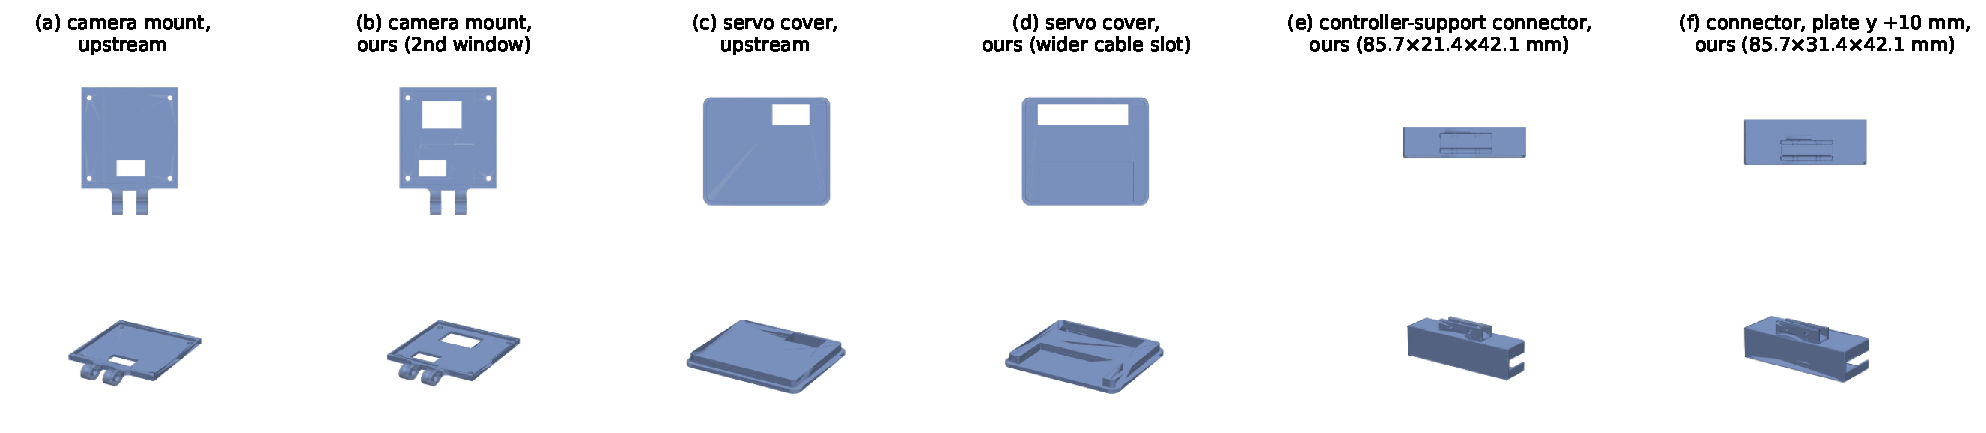
\includegraphics[width=\textwidth]{../figures/fig10_handumi_mods.pdf}
\caption{Our changes to the upstream HandUMI parts (renders of the printed meshes). (a,b) camera mount: a second window cut
above the existing one; (c,d) servo controller cover: the cable opening widened; (e) the new left controller-support connector
that replaces the upstream VR-controller support; (f) its clamp plate lengthened by 10\mm, the current version.}
\label{p1:fig:hwmods}
\end{figure*}

\section{Dataset and Task Design}\label{p1:sec:data}
\textbf{Recording.} Each hand wears a HandUMI unit (Sec.~\ref{p1:sec:hw}): a 1920$\times$1080, 30\,fps fisheye camera, a 200\,Hz IMU and a jaw encoder
sampled at 100\,Hz. A fixed head-mounted Logitech C922 records a 640$\times$480, 30\,fps view of the table; this is the global
view given to the policy (Fig.~\ref{p1:fig:dataset}a). All streams are written to one MCAP file and three videos per episode.

\textbf{Task.} Three 50\mm cubes (red, blue, purple) are stacked on a fixed plate in one of six orders; the instruction names the
order, e.g.\ ``Stack the blue cube on the bottom, purple cube in the middle, and red cube on the top, on the plate.'' An
auto-loop records a 20\,s take after spoken cues and gives a 10\,s reset in which the operator re-places the cubes by hand.
The next order is the least-collected one (target 50 per order), so orders are \emph{balanced}, not randomized. The cube
layout varies between episodes through the manual reset, around a nominal layout matched to our robot workspace, but it
was not recorded; there is no per-episode layout label.

\textbf{Collection.} One operator recorded 349 episodes in 15 sessions over three days (15--17 September 2026), 2.20\,h in
total (median episode 23.05\,s). Per order: RBP 64, RPB 62, BRP 61, BPR 56, PRB 55, PBR 51 (Fig.~\ref{p1:fig:dataset}b). Episodes from ten early sessions (55 episodes) are tracked as a separate provenance domain (``early'') from the main 294, because
their gripper anchors were derived afterwards; after filtering the two domains behave alike.

\textbf{Calibration.} Wrist cameras use a Kannala--Brandt fisheye model (left $f_x{=}789$, right $f_x{=}791$\,px). Kalibr
camera--IMU calibration gives time offsets of 30.2 and 32.8\,ms with mean reprojection errors of 6.0 and 5.6\,px, which is
high and one reason pose accuracy is validated separately (Sec.~\ref{p1:sec:proc}). The camera-to-TCP transform is a caliper
measurement, $t=[0, 55.3, 122.5]$\mm with a fixed axis permutation, following UMI's use of a CAD constant; it was measured on
one unit and applied to both. The jaw-width scale (aperture $67.5\pm5$\mm) is estimated from video of 50\mm-cube grasps; a
caliper check is pending.

\begin{figure*}[t]
\centering
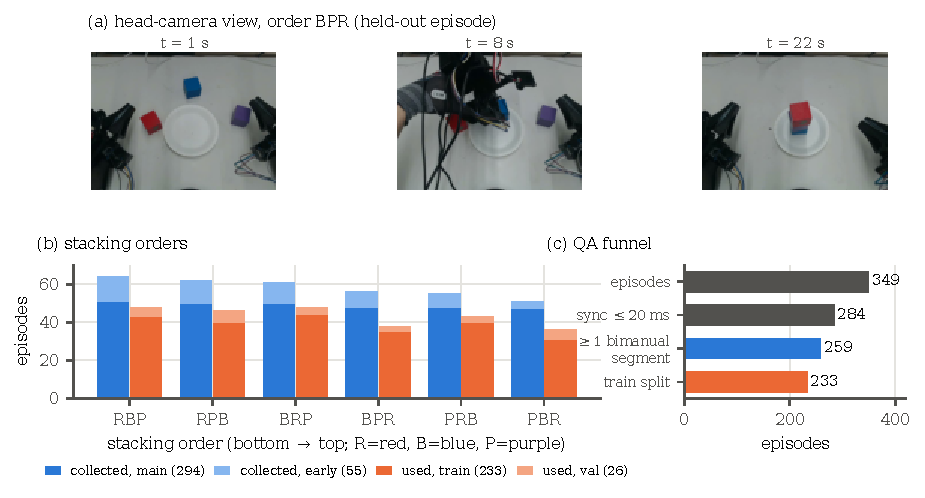
\includegraphics[width=\textwidth]{../figures/fig2_dataset.pdf}
\caption{Dataset design. (a) Head-camera frames at 1, 8 and 22\,s of a held-out episode (order BPR). (b) Episodes per stacking order, as collected
(main/early domains) and after processing (train/val). (c) Episode-level QA funnel.}
\label{p1:fig:dataset}
\end{figure*}

\section{Processing and Splits}\label{p1:sec:proc}
\textbf{Wrist poses.} UMI localizes all demonstrations in one ORB-SLAM3 map per scene. On our data this failed: maps built
before a scene change did not relocalize, and on a marker benchmark (below) its tracks cover a median of 3\% of each demonstration, with frequent position
reversals (median reversal rate 0.24 versus 0.07 for the method we adopt). We therefore run MASt3R-SLAM on the RGB wrist video alone and recover metric scale
per episode from the IMU (visual--inertial fit over a 15-frame window). On a separate benchmark of 14 ArUco-marker episodes
(28 hand trajectories; 10 held out), run on the same GPU as the dataset, this gives median tracking coverage 1.00 versus 0.03
for ORB-SLAM3 with a stored map, scale error p50/p90 of 4.6/17.0\% (versus 18.5/23.8\% for one global constant), rotation error p50/p90 0.84/2.13\textdegree{} and a UMI-style 16-step relative
position error p90 of 11.3\mm. The 349 episodes themselves have no ground truth.

\textbf{Retargeting.} Each TCP trajectory is mapped to a reBot B601 6-DoF arm by inverse kinematics on its URDF. Absolute
workspace geometry is not recoverable across episodes, so each segment is re-anchored at a fixed robot start pose (the median
active pose of our robot teleoperation data); motion is transferred, absolute cube positions are not. The jaw encoder becomes a
binary gripper command.

\textbf{Gates.} Table~\ref{p1:tab:funnel} lists the funnel. 65 episodes fail the $\le$20\,ms synchronisation requirement for a full
65-frame window; the remaining 284 yield 1{,}306 candidate bimanual segments, of which 677 leave the robot workspace, 50 fail the
metric-scale check and 18 fail IK, leaving 561 (43.0\%). Two sessions (6 episodes) were quarantined for an IMU--camera
rotation inconsistency; none contributed a segment. The training unit is a 65-frame (2.17\,s) segment; 47\% of segments start
in the first 5\,s of an episode.

\textbf{Split.} The 259 episodes with at least one bimanual segment are split at random by episode (seed 0, 10\%): 233 train /
26 val, i.e.\ 504/57 segments and 32{,}760/3{,}705 frames. No episode spans both sides. The split is not stratified; validation
has 3--6 episodes per order, 22 main / 4 early, from 9 of the 13 non-quarantined sessions.

\begin{table}[t]
\centering\footnotesize
\caption{Processing funnel (counts recomputed from the census files in the repository).}
\label{p1:tab:funnel}
\setlength{\tabcolsep}{4pt}\begin{tabular}{@{}lrr@{}}
\toprule
Stage & Episodes & Segments \\
\midrule
Recorded (KEEP) & 349 & -- \\
Pose + gripper exported (698 tracks) & 349 & -- \\
Sync $\le$20\,ms, $\ge$65-frame window & 284 & 1{,}306 \\
\quad $-$ workspace / metric scale / IK & & $-$677 / $-$50 / $-$18 \\
$\ge$1 bimanual segment (training pool) & 259 & 561 \\
\quad train / val (by episode, seed 0) & 233 / 26 & 504 / 57 \\
\bottomrule
\end{tabular}
\end{table}

\section{Model and Training}\label{p1:sec:model}
We fine-tune X-VLA~\cite{zheng2025xvla} (LeRobot implementation) from the public \texttt{xvla-base} checkpoint: a Florence-2
vision-language encoder~\cite{xiao2024florence2} and a 24-layer transformer policy (hidden 1024, 16 heads, 32 soft prompts) with a
flow-matching action head (10 denoising steps); 879M parameters, all trainable. Inputs are the three views (head, left wrist,
right wrist; resized to 224\,px), the order instruction and a 14-D state (6 joint angles and a binary gripper per arm).

\textbf{Action target.} For state time $t$ the model predicts a 30-step chunk $a_i = q_{t+5+i}-q_t$, $i=0,\dots,29$, of
cumulative joint displacements of the retargeted pseudo-joints (a 5-frame lead, so the chunk covers 0.2--1.17\,s ahead), plus
the absolute gripper command. Two auxiliary terms tie joint space to the measured human motion: (C) the relative TCP position
of the measured trajectory, predicted in spare action dimensions (weight 2.0), and (D) a forward-kinematics loss between
$\mathrm{FK}(q_t+\hat a_i)$ and the measured TCP position (weight 20). Targets are the measured human transitions, never
relabelled robot commands.

\textbf{Optimization.} 300k steps, batch 4, AdamW (lr $10^{-4}$, weight decay $10^{-4}$, 1k warm-up, cosine decay to
$2.5\times10^{-6}$), gradient clipping 10, fp32, one RTX~4090. A checkpoint is saved every 10k steps.
The checkpoint selection rule, minimum geo score (below) on all validation samples, was fixed before training.

\section{Evaluation Protocol}\label{p1:sec:eval}
Evaluation is open-loop on the 26 held-out episodes: from each of the 57 validation segments we take 7 start frames (every 5
frames in 0--30), giving 399 samples and 798 arm-samples, and compare the predicted chunk against the recorded future.
For horizons $k\in\{1,4,8,16,30\}$ we report the TCP position error between $\mathrm{FK}(q_t+\hat a_k)$ and the measured TCP
(median, mm), the joint MAE and that of a \emph{zero-motion} predictor ($\hat a\equiv0$), and the cosine between predicted and
measured TCP displacement. The \emph{geo score} is the mean of the median TCP error over the five horizons. Because most samples
are near-static, we also report every metric on the \emph{moving} subset, arm-samples whose measured TCP moves $\ge$20\mm by $k{=}30$
(187 of 798, 23.4\%). This gate was added after the 60k checkpoint had been evaluated and is used for reporting only.

\textbf{Prompt swap.} To test instruction use, we query the final checkpoint on every sample with each of the six order
instructions using the same noise seed, and with the true instruction under two further seeds. The spread of the six
predictions measures the instruction's effect; the spread across seeds is the sampling-noise floor.

\textbf{What the split does not test.} Validation episodes share operator, scene, sessions and all six orders with training,
and layouts are unlabelled. The results therefore measure within-distribution generalization to new \emph{episodes}, not to new
layouts, orders or scenes.

\section{Results}\label{p1:sec:results}
\begin{table*}[t]
\centering\footnotesize
\setlength{\tabcolsep}{7pt}
\caption{Offline held-out results (26 episodes). TCP error: median FK position error (mm); MAE: joint MAE (deg), with the
zero-motion predictor in parentheses; cos: TCP direction cosine. 160k is the pre-registered selection, 300k the final step.}
\label{p1:tab:results}
\begin{tabular}{@{}llccccc@{}}
\toprule
 & & \multicolumn{5}{c}{horizon $k$ (steps of 1/30\,s after a 5-frame lead)} \\
\cmidrule(l){3-7}
Subset & Metric & 1 & 4 & 8 & 16 & 30 \\
\midrule
\multirow{3}{*}{All (798)} & TCP err., 160k & 1.3 & 1.7 & 2.2 & 3.1 & 5.7 \\
 & TCP err., 300k & 1.5 & 1.8 & 2.2 & 3.2 & 5.7 \\
 & MAE, 300k & 0.30 (0.15) & 0.34 (0.19) & 0.42 (0.25) & 0.57 (0.36) & 0.97 (0.51) \\
\midrule
\multirow{4}{*}{Moving (187)} & TCP err., 160k & 11.2 & 15.0 & 19.9 & 29.2 & 39.1 \\
 & TCP err., 300k & 11.2 & 15.0 & 19.4 & 29.3 & 39.9 \\
 & MAE, 300k & 2.02 (2.32) & 2.68 (3.36) & 3.29 (4.38) & 4.30 (6.34) & 6.59 (8.68) \\
 & cos, 300k & 0.72 & 0.80 & 0.84 & 0.86 & 0.90 \\
\bottomrule
\end{tabular}
\end{table*}

Table~\ref{p1:tab:results} and Fig.~\ref{p1:fig:eval} summarize the evaluation. Four findings stand out.

\textbf{(1) Aggregate errors mostly reflect static phases.} The geo score reaches 2.78\mm at 160k and 2.88\mm at 300k and is
flat after about 120k (Fig.~\ref{p1:fig:eval}a). On moving samples, however, the error is an order of magnitude larger: 11\mm at the
shortest horizon and 40\mm at $k{=}30$, with a p90 of 90\mm; the moving-subset geo score is 23.0\mm versus 2.9\mm on all
samples.

\textbf{(2) On moving samples the policy predicts the direction of motion and beats a no-motion baseline.} The direction
cosine rises from 0.72 at $k{=}1$ to 0.90 at $k{=}30$, and joint MAE is 13--32\% lower than the zero-motion predictor across
horizons (6.59 versus 8.68\textdegree{} at $k{=}30$; Fig.~\ref{p1:fig:eval}b). The model captures the direction of the upcoming motion, not only its presence.

\textbf{(3) On all samples, the policy is worse than predicting no motion.} Joint MAE is about twice the zero-motion MAE at
every horizon (0.30 versus 0.15\textdegree{} at $k{=}1$): during static phases the policy predicts small spurious motion, and the
median predicted-to-measured displacement ratio is 1.41 at $k{=}1$. At $k{=}30$ the spread of predictions is 0.77 of the spread
of targets, so the long horizon is somewhat under-dispersed rather than collapsed.

\textbf{(4) The order instruction changes predictions but does not improve them.} In the prompt swap
(Fig.~\ref{p1:fig:eval}c), the six instructions move the predicted TCP by a median of 4.8\mm at $k{=}30$ on moving samples, about
50$\times$ the sampling-noise spread (0.09\mm) but only 8\% of the predicted displacement (62\mm). The true instruction is not
closer to the recorded motion than the wrong ones: its error is 39.9\mm versus 39.5\mm for the mean wrong instruction, and its
mean rank among the six is 3.55 (chance 3.5; rank 1 in 16\% of cases, chance 17\%), with the same picture at every horizon and
on all samples. The prediction with the true instruction and the original seed reproduces the reference evaluation to within
$10^{-5}$\mm. A caveat is that much of a 2.2\,s segment is order-independent (reaching, lifting); a test restricted to
choice points (the first reach of an episode) needs more such samples than the 26 validation episodes provide.

Per-order breakdowns are in the repository; with 3--6 validation episodes per order they are too small to rank orders, and we do
not interpret differences between them.

\begin{figure*}[t]
\centering
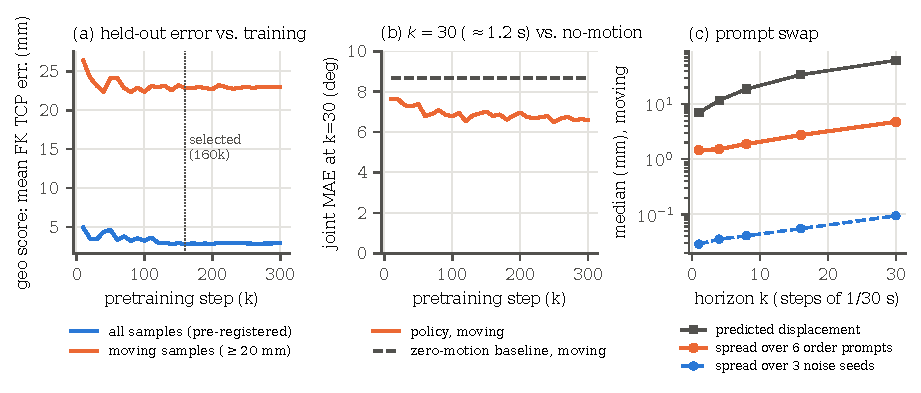
\includegraphics[width=\textwidth]{../figures/fig4_eval.pdf}
\caption{Offline evaluation. (a) Geo score over training on all versus moving held-out samples; the pre-registered rule
selects 160k. (b) Joint MAE at $k{=}30$ on moving samples, policy versus zero-motion predictor. (c) Prompt swap on the final
checkpoint: prediction spread across the six order instructions (same seed) versus across three noise seeds (true instruction).}
\label{p1:fig:eval}
\end{figure*}

\section{Failure Analysis}\label{p1:sec:fail}
\textbf{Weak use of the task-order instruction.} The order prompt measurably changes the prediction, but this variation does
not improve agreement with the recorded motion (finding 4).
In this dataset the order is also partly visible from the scene once stacking has begun, so the instruction is only necessary
at the start of an episode; nothing in training forces the model to use it.

\textbf{Static-phase drift.} The dominant error mode is non-zero motion predicted while the human is still. It is the reason
the all-samples MAE exceeds the zero-motion baseline, and on a robot it would appear as creep before grasps or after placement.
One plausible contributor, not yet tested, is residual pose noise in near-static windows, which makes ``stationary'' targets noisy.

\textbf{Long-horizon under-dispersion.} Predictions at $k{=}30$ vary less than the targets (ratio 0.77) and the p90 error on
moving samples reaches 90\mm, so fast or unusual motions are pulled towards the mean.

\textbf{Data lost before learning.} 57\% of the candidate segments are removed; the workspace gate accounts for 677 of the 745
removals (91\%), and in 531 of those (78\%) only one arm leaves the robot workspace. Because the gate removes motions by
their extent, the kept set is likely biased towards compact motions; we have not yet quantified this bias.

\textbf{Upstream failures that shaped the design.} ORB-SLAM3 with a stored map failed to relocalize across scene changes and
produced position jitter; a camera-orientation convention error in an earlier export corrupted rotations until it was found by a frame-regression test; and 65 episodes (19\%) fail synchronisation. Each was found by an explicit gate,
not by training loss.

\section{Follow-up Experiments}\label{p1:sec:follow}
\textbf{Retargeting v2.} The single start anchor of Sec.~\ref{p1:sec:proc} was the main source of loss: every segment began at
one robot posture, so most left the workspace and the retargeted joint trajectories covered one posture cluster. We replaced
it with multi-seed retargeting under a strict budget: every real-robot quantity (seed bank, workspace gate, posture
penalty, trajectory windows) comes from 30 robot episodes only, and results are measured against a disjoint set of 120
robot episodes. Table~\ref{p1:tab:retarget} compares four variants on the same 1{,}229 candidate segments. Trajectory-window
retrieval (TR), which starts each human segment from the closest feasible robot trajectory window, is the most
robot-like: posture distance to the held-out robot data falls from 1.49 to 0.27\,rad (median) and start postures span 100
clusters instead of 1. It solves fewer segments than the kinematic variants because it cannot place fast motions; among the
686 segments both TR and the penalised kinematic variant solve, their joint-velocity distributions are similar (W1 0.00207
vs 0.00226), so the posture gain, not a dynamics gain, is what TR adds. The remaining failures are almost all ``no
workspace-compatible window'' (399 of 402 unsolved).

\begin{table}[t]
\centering\footnotesize\setlength{\tabcolsep}{3.5pt}
\caption{Retargeting variants on the 1{,}229 candidate segments of the 259 episodes, measured against 120 held-out robot
episodes. NN: nearest-neighbour joint-space distance to robot postures (rad, p50/p90); W1: Wasserstein distance of
$|\Delta q|$ per step.}
\label{p1:tab:retarget}
\begin{tabular}{@{}lcccc@{}}
\toprule
Variant & Usable & NN p50 / p90 & Start clusters & W1 $|\Delta q|$ \\
\midrule
v1 single anchor & 36.5\% & 1.49 / 1.55 & 1 & 0.00197 \\
v2-K multi-seed IK & 66.6\% & 1.21 / 1.60 & -- & 0.00275 \\
v2-Kr + posture penalty & 67.0\% & 0.44 / 0.74 & -- & 0.00310 \\
v2-TR window retrieval & 56.1\% & 0.27 / 0.45 & 100 & 0.00208 \\
\bottomrule
\end{tabular}
\end{table}

\textbf{Robot-like re-collection.} To test whether the loss is a collection-style problem, we added a robot-like protocol to
the collector (30\,s takes, live wrist-rotation speed and grasp feedback against robot statistics) and recorded 60 new
episodes (10 per order) in one session. Its interpretation rules were fixed before retargeting. Live rotation speed halved
(median over-threshold fraction 0.144 to 0.067), but the per-episode TR yield did not change (0.59 vs 0.59) and TR usable
rose only from 56.1\% to 58.9\%; the per-episode correlation between live robot-likeness and TR yield is weak
(Spearman $\rho=-0.11$, $p=0.05$, pooled $n=316$). Robot-like movement, as measured live, is associated with, but not a
proxy for, retarget feasibility; workspace placement remains the main failure. The final TR dataset combines both
collections: 996 segments (896 train / 100 val) from 316 source episodes, with the original 689 segments preserved
bit-identically.

\textbf{Ego pretraining for robot fine-tuning.} The first-release ego checkpoint (Sec.~\ref{p1:sec:model}) and the base
checkpoint were each fine-tuned on 150 robot teleoperation episodes of the same task with the same recipe, data and
evaluation; only the initialization differs. At the matched step of 250k, the ego-initialized model has a 10.0\% lower geo
score (episode-level paired bootstrap, 10k draws: 95\% CI $-14.7$ to $-5.6\%$), a 7.2\% lower moving-sample geo score (CI
$-13.4$ to $-1.8\%$) and 6.8\% lower moving joint MAE at $k{=}30$ (CI $-12.7$ to $+0.5\%$); 8 of the 10 evaluation
episodes favour it. The evaluation episodes are part of both fine-tuning sets, so this measures how well each model fits
the robot training distribution, not generalization. A smaller-data comparison on 90 robot episodes was stopped early with
only two matched steps (10k, 20k); there the signs are mixed (all-sample geo $-33\%$ and $-11\%$, moving-sample geo $+2\%$ and
$+13\%$ for the ego initialization), so we draw no conclusion from it.

\textbf{Pretraining on the final dataset.} X-VLA was pretrained from \texttt{xvla-base} on the 996-segment dataset with
the same recipe (planned 300k steps). The run was stopped at 211.7k steps; the 100k and 200k checkpoints are kept, with 100k
designated as the initialization for later robot fine-tuning. No robot fine-tuning result from these checkpoints is
reported here: the only fine-tuning comparison above uses the first-release ego checkpoint.

\section{Cartesian Ego Data (v3)}\label{p1:sec:v3}
Retargeting to robot joints (Secs.~\ref{p1:sec:proc} and \ref{p1:sec:follow}) had two costs: the workspace and IK gates removed a third
to a half of the candidate motion, and the joint-space target differed from the Cartesian action space our robot policies are
fine-tuned in. Version 3 drops the pseudo-joint step. Each human wrist trajectory is converted directly into the same
relative end-effector representation as the robot teleoperation data, so that ego and robot samples share one tensor contract
and differ only in where they came from.

\textbf{Contract.} Rows are stored at 15\,Hz. For row time $t$ the action is a chunk of 16 future poses
$A_k = T(t)^{-1}\,T(t + k\Delta)$, $k=1..16$, with $\Delta = 50.05$\,ms (the robot data's step, 0.80\,s in total), interpolated on
the raw 30\,Hz track (linear in position, SLERP in rotation) rather than taken from neighbouring rows. Each arm contributes
position, a 6-D rotation and a gripper value (20 dimensions for two arms, ``CART20''); the model's 32-D action is padded with 12
dimensions that are exactly zero and never supervised. The state is each arm's pose relative to its own task-start pose plus
the two gripper values, the same layout as the robot state. The gripper is the continuous jaw aperture divided by 80\mm; the
largest observed value is 0.847, so the ``fully open'' end is never reached. A row is kept only if both arms are valid at $t$,
all 16 targets lie on valid raw samples no more than 50\,ms apart, and a head-camera frame exists within 20\,ms; there is no
padding. Eleven synthetic tests pin the contract. Fig.~\ref{p1:fig:traj} shows the wrist trajectories that the labels are
cut from; the full videos are in the repository.

\begin{figure*}[t]
\centering
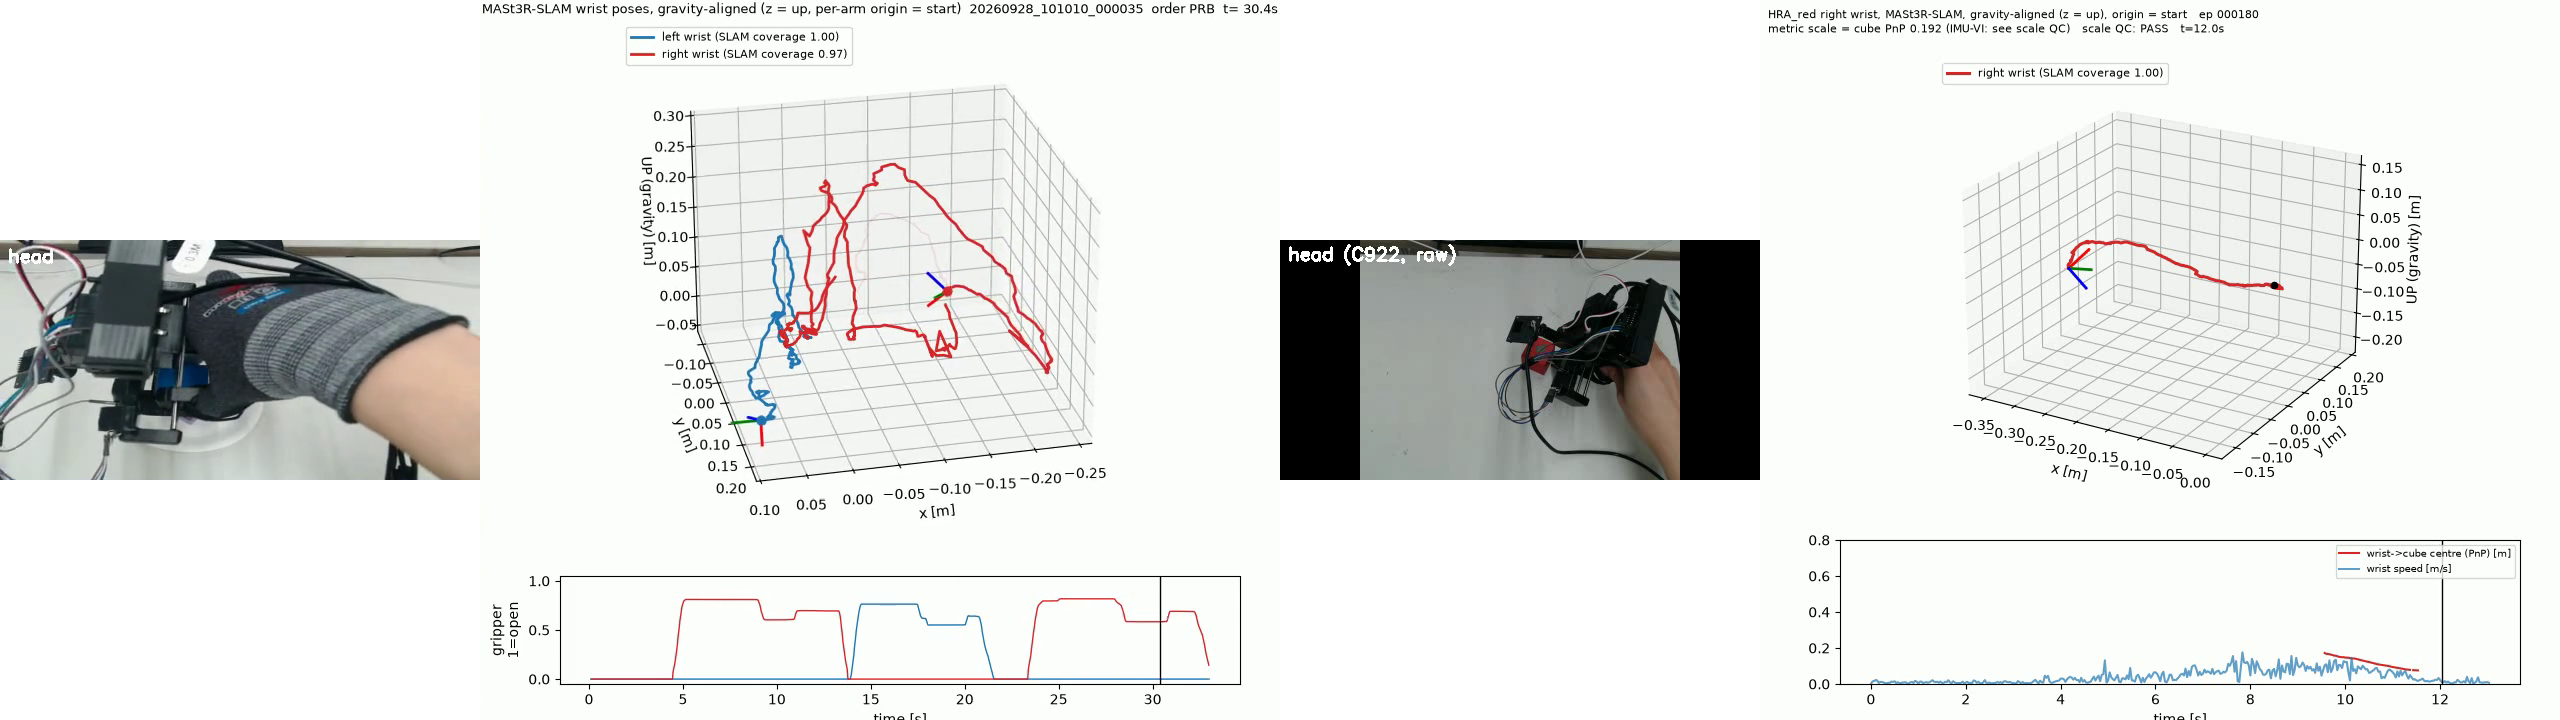
\includegraphics[width=0.8\textwidth]{../figures/fig7_mast3r_trajectories.png}
\caption{MASt3R-SLAM wrist trajectories of an HRL80 stacking take (order PRB). Left: head camera and both wrist fisheye
cameras. Right: trajectories gravity-aligned (z up), each arm's origin at its start pose, current tool axes drawn (x red,
y green, z blue), metric scale from the IMU; below, both grippers (1 = open). Videos of three takes (PRB, RBP, PBR):
\texttt{docs/media/mast3r\_trajectories/hrl80\_0000\{35,55,60\}\_wrist.mp4} in the repository.}
\label{p1:fig:traj}
\end{figure*}

\textbf{Data.} The source is the 273 original episodes that have valid per-hand IMU scale and 60 HRL80 episodes; 3 HRL80 episodes
are refused because one hand's IMU scale is invalid, leaving 330. Nothing is filtered for robot workspace or IK feasibility.
Of 111{,}533 rows at 15\,Hz, 57{,}283 (51.4\%) are usable for training; the rest fall on tracking losses, synchronisation gaps
or the last 0.8\,s of an episode. The split is frozen from the earlier releases (validation = the 26 held-out episodes of
Sec.~\ref{p1:sec:proc} plus HRL80 episodes 49--54): 298 train episodes with 51{,}612 rows and 32 validation episodes with 5{,}671 rows.

\textbf{Silent pose jumps.} Comparing ego and robot state statistics showed per-row state jumps above 100\mm in the ego data
that the robot data does not have. Two causes were mixed. First, the exported dataset contains only training rows, so
``adjacent'' frames can be seconds apart: 1{,}482 of the 2{,}598 apparent jumps above 30\mm (57\%) are such time gaps, and
adjacency has to be decided from row timestamps. Second, the remaining jumps are real: MASt3R-SLAM occasionally moves the
camera by 10\,cm or more within one 30\,Hz frame without flagging tracking loss (55 raw steps faster than 3\,m/s in 24 training
episodes, none preceded by a loss flag). Because the state is anchored at task start, a one-way jump corrupts every later
state of that episode, while the current-anchored action is affected only for 0.8\,s. The v2b filter drops the remainder of an
episode after a one-way jump (above 100\mm or 45\textdegree{} per row, or an isolated step above 50\mm between two slow steps)
and drops isolated spikes only. It acts on 44 events in 42 training episodes and removes one episode entirely; training
shrinks to 297 episodes and 48{,}411 rows ($-6.20$\%), validation is unchanged. The largest step between time-adjacent rows
falls from 422.5 to 90.5\mm and steps above 100\mm from 18 to 0; 7 raw steps faster than 3\,m/s remain inside valid rows.

\textbf{How ego data differs from robot data.} On 60 ego and 60 robot episodes, with the ego poses attached to a robot start
pose: the robot's IK reaches 99.7\% (left) and 99.5\% (right) of ego positions, and 72.3\%/74.6\% of full ego poses. The IK
configuration used on the robot, which locks one wrist joint, reproduces only 45.2\%/52.2\% of the robot's \emph{own} recorded
poses, a deployment limitation that exists without any human data. Ego hands use a smaller workspace (state p95 0.221/0.214\,m
versus 0.395/0.369\,m) with similar 0.4\,s translations (p95 93/99 versus 91/100\mm), and both ego hands are still at the same
time far more often (19.5\% versus 2.4\% of samples at 0.4\,s). The largest difference is visual: the variance of the image
Laplacian, a sharpness measure, has a median of 1{,}854/1{,}487 for the ego wrist fisheye views and 59/64 for the robot's wrist
cameras.

\section{Transfer Experiments}\label{p1:sec:transfer}
All runs in this section share one recipe: X-VLA with the 32-D action head, loss on action dimensions 0--19 only, dimensions
20--31 zeroed at input and output, batch 8, 8-bit AdamW (policy learning rate $10^{-4}$, warm-up 1k, cosine decay ending at the
last step), bf16 mixed precision, seed 1000. Robot data is R312c, 312 teleoperated episodes (174{,}012 frames) of the same
six-order stacking task. Fine-tuning starts a fresh optimizer and uses robot normalization statistics.

\textbf{Which soft prompt?} X-VLA conditions on a dataset/embodiment id that selects a set of soft prompts. Our earlier runs used
id~0. Reading the public base weights shows that only slots 10--17 were trained: in the other 22 slots the encoder and decoder
biases are exactly zero and the prompt weights stay near their initialization. Ids 0 and 6, both used by us, were therefore untrained
slots. The trained slots are not a better start either: the initial loss on R312c is 1.11 for slot 0, 1.12 for 6, 1.61 for 15,
2.35 for 10, 2.65 for 16, 4.07 for 17 and 22.80 for 11. All runs below use the unused slot 20 as our embodiment's own slot.

\textbf{Ego-only model on robot frames.} After 40k steps on ego data alone, the model was queried, teacher-forced, on 120 robot
frames and compared with a model trained 40k steps on robot data (these frames are in that model's training set, so its value
is an upper reference). The median cosine between predicted and recorded translation at 0.4\,s is $+0.81$/$+0.77$ (left/right)
for the robot model and $-0.05$/$-0.03$ for the ego model. No combination of a left/right swap and axis sign flips raises the ego
model above $+0.16$, and the wrist-camera optical flow has the same sign relations to TCP motion in both domains, so this is not
a convention error.

\begin{table}[t]
\centering\footnotesize\setlength{\tabcolsep}{3.2pt}
\caption{Ego-only checkpoint (40k), median direction cosine at $k{=}4/8/16$ (left $|$ right) when images and state come from
different domains. 100 ego validation frames and 100 robot frames; 21--55 moving frames per cell.}
\label{p1:tab:ablation}
\begin{tabular}{@{}lcc@{}}
\toprule
Images + state & Left $k$=4/8/16 & Right $k$=4/8/16 \\
\midrule
ego + ego & 0.87 / 0.91 / 0.92 & 0.89 / 0.94 / 0.84 \\
ego + zero & 0.77 / 0.80 / 0.89 & 0.85 / 0.80 / 0.66 \\
ego + robot & 0.76 / 0.81 / 0.90 & 0.72 / 0.69 / 0.72 \\
robot + robot & 0.36 / 0.30 / $-$0.01 & 0.19 / 0.02 / $-$0.15 \\
robot + zero & 0.17 / 0.25 / $-$0.25 & 0.24 / 0.06 / $-$0.02 \\
robot + ego & 0.16 / 0.24 / $-$0.16 & 0.49 / 0.33 / $-$0.03 \\
\bottomrule
\end{tabular}
\end{table}

\textbf{The gap is in the images.} Table~\ref{p1:tab:ablation} swaps the two inputs. With ego images the model keeps a cosine of
0.69--0.90 whatever state it is given, robot state included; with robot images it falls to between $-0.25$ and $+0.49$ whatever
the state. The failure is visual, which fits the 30-fold sharpness difference of the wrist views.

\textbf{Ego pretraining as an initialization.} We fine-tuned on R312c from the base model (A) and from the ego model after 50k
steps (B), with identical data, schedule (150k-step cosine), seed and recipe; both were stopped by us near 60k. At step 200 the
training loss is 0.945 for A and 0.244 for B. The ratio B/A is 0.49 over the first 5k steps, 0.875 over 5k--20k and 0.95 over
20k--40k, and over 55k--60k the two are tied (0.0733 versus 0.0745; B lower at 13 of 24 logged points)
(Fig.~\ref{p1:fig:egoinit}). Ego pretraining therefore speeds up early fitting of the robot data and gives no measurable advantage
in training loss by 60k. This is training loss with one seed per arm; we have no held-out or closed-loop comparison of A and B.
Two 300k runs finished later, but on different robot datasets (R312c for the ego-initialized run, 384 episodes for the
scratch run), so they are not a transfer comparison and we do not report one.

\begin{figure*}[t]
\centering
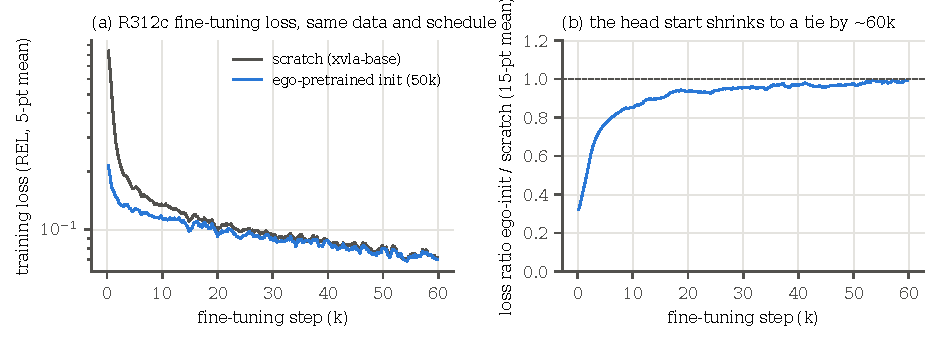
\includegraphics[width=\textwidth]{../figures/fig5_ego_init_loss.pdf}
\caption{R312c fine-tuning from the base model versus from the 50k ego checkpoint, same data, schedule and seed. (a) Training
loss. (b) Ratio of the two; values below 1 favour the ego initialization. Training loss only.}
\label{p1:fig:egoinit}
\end{figure*}

\textbf{Attempts to close the visual gap.} To make the ego wrist views look like the robot's, we re-render each fisheye frame as a
virtual pinhole camera (62--70\textdegree{} horizontal field of view, principal point shifted so that the jaws sit low in the
image as on the robot), then downsample, blur and JPEG-compress it. Labels, state and head images are unchanged. Applied to
every frame (ROBOT100) the wrist sharpness median drops from 1{,}854/1{,}487 to 181/132, still two to three times the robot's
59/64. A run with 70\% of frames re-rendered was stopped at 5k steps; a co-training run with exactly four ego (ROBOT100) and
four robot samples per batch was stopped at 88.6k steps without evaluation. A 300k ROBOT100 pretraining run (297 episodes,
48{,}411 rows, 49.6 epochs) finished on 5 October at a training loss of 0.007; its checkpoints are the ego initializations of
Sec.~\ref{p1:sec:r30}. No offline transfer metric was computed for the re-rendered models.

\textbf{On the robot.} Checkpoints from every run above were executed on the reBot through our deployment interface: 71
checkpoints, 49{,}431 control cycles and 1{,}681 run starts between 2 and 4 October. The cycle log records IK tracking of the
model's own waypoints, not task outcome, and has no episode or instruction field, so it yields no success rate. Two
operator observations were not logged. First, the ego-initialized model at 10k fine-tuning steps grasped cubes but picked
the wrong colour. Second, the ego-initialized model fine-tuned on R312c for 300k (B300, checkpoints between 75k and 205k)
completed the full three-cube stack on the robot in closed loop. The number of trials was not recorded and no video was
taken, so we state only that closed-loop three-cube stacking has been demonstrated, with no success rate. It also says
nothing about the value of ego pretraining: no scratch model trained on the same R312c data was evaluated under the same
protocol (the finished scratch 300k run used R384). Between 5 and 7 October the only bimanual robot use was one short run of
the R384 scratch model (200k, 4 control cycles). A trial logger with the fields listed in Sec.~\ref{p1:sec:lim} was added to the
deployment interface on 4 October but has not been used, so there are still no logged trial outcomes. During a storage clean-up
on 4 October only checkpoints at multiples of 50k were kept; of the B300 checkpoints that stacked, 150k and 200k survive and
the others (155k--205k) are gone, so the demonstration can be re-run only from 150k or 200k.

\section{Low-Data Ablation: 30 Robot Episodes}\label{p1:sec:r30}
The 312-episode comparison of Sec.~\ref{p1:sec:transfer} gives the robot data every chance to wash out the initialization. The
question that matters for using human data is whether it helps when robot data is scarce. We therefore fine-tuned on R30,
episodes 150--179 of R312c (30 episodes, 17{,}600 frames, five per stacking order), with the recipe of
Sec.~\ref{p1:sec:transfer}, R312c normalization statistics, seed 1000 and a 600k-step cosine schedule, from three
initializations: the base model (scratch), and the ROBOT100 ego pretraining run of Sec.~\ref{p1:sec:transfer} at 100k and at
300k steps. The 100k checkpoint is taken from the middle of the same 300k-step schedule, so its learning rate had not decayed;
it is not a separate 100k-step run. The two ego arms also ran on different machines (scratch and 100k-init on an RTX~4090
with PyTorch~2.6, 300k-init on an RTX~5090 with PyTorch~2.7.1), so they are not bit-identical twins.

\begin{table}[t]
\centering\footnotesize\setlength{\tabcolsep}{4pt}
\caption{R30 fine-tuning, training loss (200-step running mean) at matched steps, and the ratio of window means to scratch
(below 1 favours the ego initialization). One seed per arm; no held-out or robot evaluation.}
\label{p1:tab:r30}
\begin{tabular}{@{}lccc@{}}
\toprule
Step & Scratch & Ego-PT 100k init & Ego-PT 300k init \\
\midrule
200 & 0.801 & 0.239 & 0.446 \\
1k & 0.312 & 0.103 & 0.117 \\
10k & 0.065 & 0.056 & 0.040 \\
50k & 0.019 & 0.017 & 0.014 \\
100k & 0.009 & 0.009 & 0.007 \\
\midrule
Window & & ratio & ratio \\
\midrule
1k--5k & & 0.544 & 0.493 \\
10k--20k & & 0.823 & 0.697 \\
50k--100k & & 0.970 & 0.856 \\
100k--150k & & 1.021 & 0.914 \\
\bottomrule
\end{tabular}
\end{table}

\textbf{Result.} Table~\ref{p1:tab:r30} and Fig.~\ref{p1:fig:r30} show the same pattern as the 312-episode comparison, stretched
out. Both ego initializations start at less than half the scratch loss (window ratio 0.54 and 0.49 over 1k--5k). The
100k-step initialization loses its advantage by about 100k steps (ratio 0.97 over 50k--100k, 1.02 over 100k--150k); the
300k-step one keeps a smaller advantage longer (0.86 and 0.91) and reaches parity at about 200k. Beyond about 150k all losses
are 0.001--0.004 at the printed precision and ratios are not meaningful. The 100k-step initialization starts lower than the
300k-step one (0.239 versus 0.446 at step 200) although it was pretrained less; we have not explained this. All three runs
were stopped by us to free GPUs, at 471k (scratch), 305k (100k-init) and 310k (300k-init), after 214, 139 and 141 epochs: with
30 episodes, every arm fits its training data almost exactly long before the schedule ends.

\textbf{What this does and does not show.} Training loss on 30 episodes measures how fast each initialization memorizes the
robot data, not how well it acts. Because all arms overfit heavily, the relevant comparison is closed-loop at early and
middle checkpoints (roughly 10k--150k), where the initializations still differ; no R30 checkpoint has been run on the robot
yet, and there is no held-out robot evaluation. The prediction that this experiment can test is whether the earlier fit of
the ego-initialized models turns into stacking at fewer fine-tuning steps; the experiment has not been done.

\begin{figure*}[t]
\centering
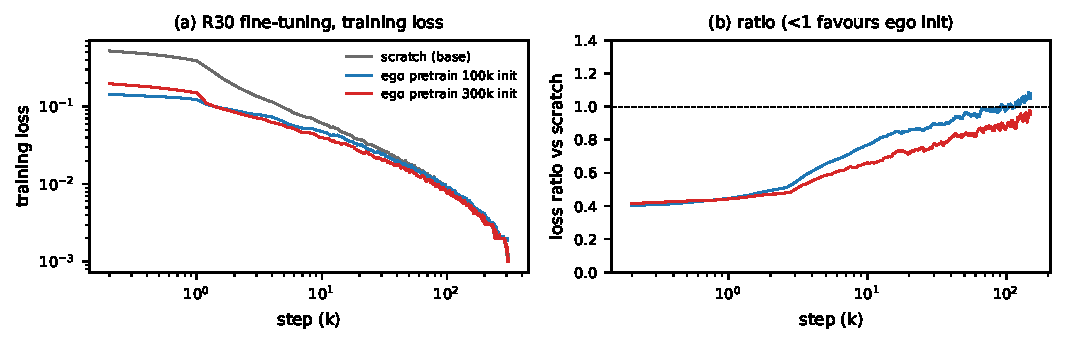
\includegraphics[width=0.8\textwidth]{../figures/fig8_r30_ablation.pdf}
\caption{R30 fine-tuning (30 robot episodes) from the base model and from ego pretraining at 100k and 300k steps. (a) Training
loss (log--log, smoothed). (b) Ratio to scratch, shown to 150k; beyond that the 3-decimal losses make the ratio noise.
Training loss only, one seed per arm.}
\label{p1:fig:r30}
\end{figure*}

\section{Lessons}\label{p1:sec:lessons}
Four findings changed how we work, and each was found by an explicit check rather than by a loss curve. (i) A pretrained
model's conditioning interface has to be audited, not assumed: two of our embodiment ids pointed at soft prompts that had never
been trained. (ii) When human and robot data share a tensor contract, the remaining gap can be localized by swapping inputs
between domains; here it is the wrist images, not kinematics or normalization. (iii) Each scale or pose source has a regime in
which it fails silently: MASt3R-SLAM on rare one-frame jumps here, and IMU scale on slow motion in Part II. Both were caught only
by comparison with an independent reference (robot statistics, a known object), which we now build into every new collection.
(iv) Training-loss comparisons of initializations end in a tie whenever the robot data is fitted to near zero, at 312 and at
30 episodes alike; only held-out or closed-loop evaluation at early checkpoints can show a benefit, and the logging for it has
to exist before the robot runs, not after.

\section{Limitations and Future Work}\label{p1:sec:lim}
\textbf{Completed:} dataset collection and calibration; the pose, retargeting and QA pipeline; 300k-step ego fine-tuning and
offline evaluation on held-out episodes; retargeting v2, the robot-like re-collection and the matched 150-episode robot
fine-tuning comparison; pretraining on the final 996-segment dataset (stopped at 211.7k steps, checkpoints 100k and 200k).
Version 3 added the Cartesian ego dataset and its filters, the soft-prompt audit, the domain-swap diagnostics, the matched
initialization comparison up to 60k steps and the robot-like wrist re-rendering. Version 4 added the finished ROBOT100
pretraining and the three-arm R30 ablation (training loss, stopped at 305k--471k). \textbf{Stopped early, no conclusion:} the
90-, 60- and 30-episode robot fine-tuning comparisons of version 2 (at most two matched steps, or only one arm run); the
70\%-re-rendered pretraining (5k steps) and the ego/robot co-training run (88.6k steps, never evaluated).
\textbf{Not yet done:} robot fine-tuning from the 996-segment checkpoints; any robot or held-out evaluation of the R30 arms;
a held-out or closed-loop comparison of the ego-initialized and scratch models; outcome logging on the robot (the logger
exists but has recorded no trial). The version-2 robot evaluation episodes overlap the
fine-tuning data, so a benefit on disjoint robot data remains to be shown.

\textbf{Not supported by this study:} (i) a closed-loop success rate (three-cube stacking was demonstrated once fine-tuned on 312 robot episodes, but trials were
not counted), or any closed-loop difference between ego-initialized and scratch models; (ii) generalization to new cube layouts, since layouts
were not recorded and absolute geometry is discarded by design; (iii) generalization to unseen stacking orders, since all six
orders appear in training; (iv) transfer beyond one operator, one scene and three days; (v) any benefit of human data for robot learning beyond fitting the robot training distribution faster; (vi) that the
ego-only policy, or the re-rendered wrist images, transfer to robot cameras. \textbf{Planned experiments:} log every robot trial (model, checkpoint, robot data size, layout, instruction, stack
level 0--3, wrong colour, failure reason) and run 20--30 trials per model; compare scratch and ego-initialized models at
matched fine-tuning steps and at reduced robot data (30 episodes) for the step and data budget at which stacking first
succeeds; record layouts from the head camera and hold out layout regions; hold out two orders
entirely and test instruction following; train with a static-phase-aware loss or weighting; evaluate closed-loop on the robot
with the order instruction as the controlled variable.

More broadly, this work is a first step towards a research agenda in which egocentric human demonstrations provide scalable
supervision for robot policies: learning human-to-robot representations that keep task geometry and intent while discarding
embodiment detail, and evaluating them with predictive world models before execution. The present results show that the
bottleneck is as much in pose recovery, filtering and evaluation design as in the policy.

\section{Conclusion}
We collected 349 bimanual egocentric demonstrations of three-cube stacking, processed them into 561 robot joint-space segments
through a gated pipeline, and fine-tuned a 0.9B VLA on the result. Offline, on moving samples the model predicts the
direction of held-out human motion reliably (cosine 0.90 at $k{=}30$) and reduces joint-space error relative to a zero-motion
baseline (by 13--32\% across horizons); on static samples it predicts spurious motion, aggregate metrics hide this, and
swapping the order instruction does not make predictions more accurate. Multi-seed trajectory retrieval removes much of the
retargeting loss, and ego pretraining gives a small, consistent gain when fine-tuning on robot data, measured on the robot
training episodes. Converting whole episodes to the robot's Cartesian action contract keeps 330 episodes without any
feasibility filter, after a filter for silent SLAM jumps. With that contract the remaining human-to-robot gap is visual: an
ego-only model gives no useful action direction on robot camera frames, and the gap follows the wrist images, not the state.
As an initialization, ego pretraining speeds up early robot fine-tuning, and the advantage in training loss is gone by
60k steps. An ego-initialized model fine-tuned on 312 robot episodes has completed full three-cube stacks on the robot, so
the task itself is solved in closed loop; whether ego pretraining reaches that point with fewer robot episodes or fewer
fine-tuning steps is the open question. For slow single-arm motions, a known object replaces IMU scale. Spatial and
task-order generalization, a benefit on disjoint robot data, and a measured success rate require the controlled
experiments listed above. On 30 robot episodes, ego pretraining again speeds up early fitting, for longer when the
pretraining is longer, and again the training-loss advantage disappears; whether it becomes a closed-loop advantage at early
checkpoints is the next experiment.
\reportpart{Part II}{Single-Arm Approach to a Cube}{part:p2}
\partabstract{Part I showed that, once egocentric human data and robot data share one action contract, the remaining gap is visual and
geometric rather than kinematic. Part II isolates the simplest transferable behaviour: the right arm approaching a red cube,
learned from egocentric human demonstrations only. We report three iterations. (1) HRA\_red: 200 right-hand takes in which
IMU visual--inertial scale turned out to be unobservable (median 0.012, non-positive in 95 takes); scale from a 3.8\,cm cube
of known size replaces it (PnP/IMU ratio 1.06 on bimanual takes where the IMU is reliable) and 166 takes survive. A 0.9B X-VLA
model trained on them overfits from the first checkpoints (held-out loss 0.150 at 15k rising to 0.299 at 105k). On the robot
it moved towards the cube from a nearby start but dragged along the table for far cubes, and calibrating the robot
(head camera, wrist hand-eye with 0.16\,px RMS) exposed several convention errors, including an 82\mm offset between the
forward-kinematics TCP and the physical jaw tip. (2) Wrist images re-rendered with the measured robot camera model and
labels expressed as robot-TCP poses through the hand-eye transform. (3) HRA\_A100: a new protocol in which every take starts
with the gripper tip held on a taped origin that the robot has also touched, giving a shared task frame (collinearity
0.38\mm), per-episode origin yaw (error p50 0.21\textdegree) and a second scale source from the table plane (ratio to cube
PnP 0.999). A table-aware conversion keeps 86 of 107 takes with a fingertip clearance of at least 7.6\mm. Start- and
origin-anchored state give the same held-out loss (0.124 versus 0.132 at 5k), and both overfit from 5k. Robot runs used a
cube-size stop as a proximity proxy (69 of 127 sessions on the last day ended on it), but no trial outcome was logged, so we
report no success rate. Most of what we learned is about frames, scale and deployment settings, which we list with the
corrections we had to make.}
\section{Introduction}\label{p2:sec:intro}
A reaching motion towards a visible object is the first segment of almost every manipulation task and the simplest one in which human-to-robot transfer~\cite{kareer2024egomimic} can be judged by eye: the arm either moves towards the cube or it does not. Part I found that an
ego-only stacking model gives no useful action direction on robot camera frames (median cosine $-0.05$/$-0.03$), and that the
gap follows the wrist images. A single-arm approach task lets us attack that gap with far fewer confounds: one arm, one object,
no grasp, no task order. The question of Part II is: \emph{can a right-arm approach prior, learned only from egocentric human
demonstrations, move the robot towards the cube, and what has to be true of the data for that to work?}

Our contributions are: a metric-scale source for slow motions that does not depend on the IMU (Sec.~\ref{p2:sec:scale}); a
calibration chain that puts human and robot data in one task frame (Secs.~\ref{p2:sec:robotcal} and \ref{p2:sec:a100}); three
dataset generations with their training behaviour (Secs.~\ref{p2:sec:v1}--\ref{p2:sec:a100}); and the deployment settings and
corrections that turned out to matter (Secs.~\ref{p2:sec:deploy}--\ref{p2:sec:corr}). We report no success rate: the trial logger
of the deployment interface was not used during these runs.

\section{Setup}\label{p2:sec:setup}
\textbf{Device and poses.} The operator wears one HandUMI unit~\cite{handumi_hw}, a UMI-style~\cite{chi2024umi} hand-worn gripper designed and published by BrikHMP18, not by us (Part I, Sec.~III), on the right hand: a 1080p30 fisheye wrist
camera, a 200\,Hz IMU and a jaw encoder; a fixed Logitech C922 records the table. Wrist poses come from MASt3R-SLAM~\cite{murai2025mast3rslam} on the RGB
video alone; Part I describes the pipeline.

\textbf{Action contract.} We keep Part I's 20-dimensional Cartesian contract (CART20): rows at 15\,Hz, a chunk of 16 relative
poses $T(t)^{-1}T(t+k\Delta)$ with $\Delta=50.05$\,ms, position, 6-D rotation and gripper per arm. For a right-only task the
left arm is a dummy (identity pose, gripper 0) and is masked out of the loss together with the gripper (jaw unused), so 9 of the
20 dimensions are supervised. The task string is ``Approach to the red cube''.

\textbf{Model and training.} X-VLA~\cite{zheng2025xvla} (0.9B, LeRobot) with Part I's recipe: soft-prompt slot 20, batch 8, 8-bit AdamW (policy
learning rate $10^{-4}$), bf16, seed 1000, a checkpoint every 5k steps, on an RTX~4090. A 300-step smoke test verified the loss
mask: masked and padded dimensions receive exactly zero gradient and every supervised dimension a non-zero one.

\textbf{Robot.} The reBot B601 right arm with a wrist C922, driven from a Mac through a pink IK solver. On the robot the left arm
is locked and both jaws hold; the deployment interface refuses any command for them.

\section{HRA\_red: Object-Based Scale}\label{p2:sec:scale}
We recorded 200 right-hand takes of ``approach the red cube'' (10\,s each) in one session on 3 October.

\textbf{IMU scale fails on slow motion.} The per-episode visual--inertial scale that works on the stacking data is
unobservable here: the approaches are slow and smooth, so the accelerometer barely constrains it. Across the 200 takes the IMU
scale has a median of 0.012 and is zero or negative, which is physically impossible, in 95 of them (Fig.~\ref{p2:fig:cube}b).

\textbf{Scale from a known cube.} The red cube is static and has a 3.8\,cm edge. In frames where it is visible we fit its
silhouette with a two- or three-face model, or a single-face model when one face is seen within 35\textdegree{} of head-on,
solve PnP, and recover the trajectory scale in closed form from the requirement that the cube stays put. An episode is valid
with at least 10 PnP frames, a bootstrap spread of at most 10\% and a cube-centre residual of at most 2\,cm. On the bimanual
HRL80 stacking takes, where the IMU scale is reliable, 37 of 57 right-hand episodes are PnP-valid and the PnP/IMU ratio has a
median of 1.062 (p16--p84 0.959--1.274; Fig.~\ref{p2:fig:cube}a).

\begin{figure*}[t]
\centering
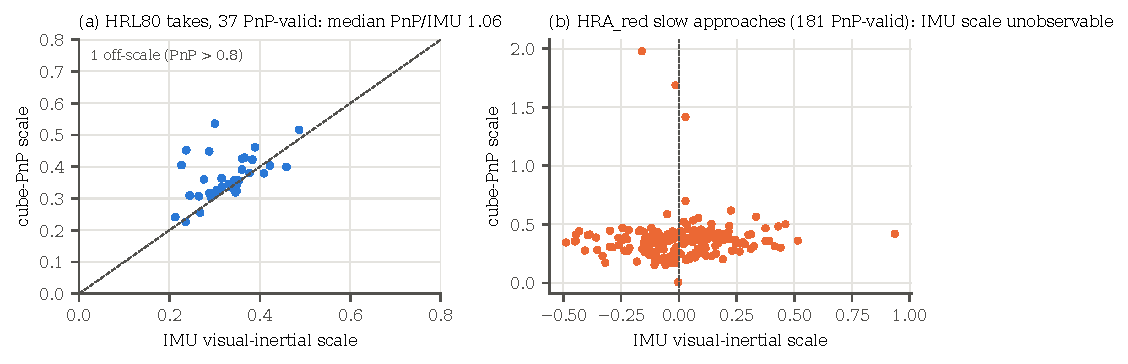
\includegraphics[width=\textwidth]{../figures/fig6_cube_scale.pdf}
\caption{Per-episode metric scale of the MASt3R-SLAM trajectory from the IMU and from cube PnP. (a) HRL80 stacking takes,
where the IMU scale is reliable. (b) HRA\_red approach takes: the IMU scale scatters around zero.}
\label{p2:fig:cube}
\end{figure*}

\textbf{Funnel.} Of 200 takes, 19 fail the scale gates (14 with too few PnP frames, 5 with too large a spread) and 15 fail a
physical sanity check on the scaled trajectory (scale between 0.1 and 1.0, SLAM travel at least 0.8 of the PnP-observed
approach distance, travel at most 0.8\,m). The remaining 166 are split into 151 train episodes (20{,}319 rows) and 15
validation episodes (2{,}011 rows). The median scale is 0.354 (p5 0.188, p95 0.500) and the median cube-centre residual 0.17\,cm.

\section{HRA\_red v1: Training and First Robot Runs}\label{p2:sec:v1}
\textbf{Training.} In v1 the wrist fisheye frames were re-rendered as a pinhole view with a \emph{guessed} robot camera
(62--70\textdegree{} horizontal field of view, principal point shifted so that the jaws sit low in the image), as for
ROBOT100 in Part I. The 300k-step run finished on 5 October at a training loss of 0.002 (118 epochs). Held-out loss rises from
the first evaluated checkpoint (Table~\ref{p2:tab:val}, Fig.~\ref{p2:fig:val}a): 0.150 at 15k (training subset 0.066), 0.198 at 30k,
0.213 at 60k, 0.265 at 90k and 0.299 at 105k, while the training-subset loss falls to 0.018. With 151 episodes the model
overfits almost immediately; checkpoints below 15k were not evaluated.

\begin{table}[t]
\centering\footnotesize\setlength{\tabcolsep}{3pt}
\caption{Held-out loss (masked MSE on the 9 supervised dimensions) by checkpoint; training-subset loss in parentheses.}
\label{p2:tab:val}
\resizebox{\columnwidth}{!}{\begin{tabular}{@{}lccccc@{}}
\toprule
Dataset (val eps) & 5k & 15k & 30k & 45k/50k & 105k \\
\midrule
HRA\_red v1 (15) & -- & 0.150 (0.066) & 0.198 (0.053) & -- & 0.299 (0.018) \\
A100 A: start (11) & 0.124 (0.110) & 0.125 (0.058) & 0.141 (0.031) & 0.224 (0.020) & -- \\
A100 B: origin (11) & 0.132 (0.097) & 0.147 (0.057) & 0.174 (0.031) & 0.190 (0.022) & -- \\
\bottomrule
\end{tabular}}
\end{table}

\textbf{First robot runs.} Checkpoints from 15k to 75k ran 8{,}397 control cycles (658 run starts) on 4 October, and v1 100k,
200k and 300k ran 61 planned sessions on the afternoon of 6 October while we tuned the chunk-execution settings
(Sec.~\ref{p2:sec:deploy}); the operator's verdicts were ``accuracy dropped a lot'' and ``too much zigzag''. From a start near
the cube the arm moved towards it; for cubes far to the left it dragged along the table, by about 39 and 26\,cm in two runs.
None of these runs has a logged outcome.

\section{Calibrating the Robot Side}\label{p2:sec:robotcal}
Interpreting those runs required knowing where the human data sits relative to the robot, which v1 never did: its labels are
relative motions of the UMI tool frame, and its start state is the human's own start.

\textbf{Head camera.} The fixed C922 (the same camera and position as during HRA\_red) was calibrated with an 8$\times$5
checkerboard of 25\mm squares (48 frames, RMS 1.05\,px, $f=728.7$\,px), and its pose in the robot base was found by touching
four board corners with the TCP (residuals 2--6\mm).

\textbf{Linking human takes to the base.} For each take we detect the cube in the head camera, place it in the robot base, and
attach the wrist trajectory through the wrist-camera cube PnP; tilt comes from IMU gravity against the table normal, yaw from
the cube faces. This linked 64 of 166 takes (head-camera detection is the bottleneck) and exposed an 18\textdegree{} rotation
error in the exported camera--IMU extrinsic (cube-axis error 17.8$\to$3.4\textdegree{} after correction); earlier IMU-based
tilt statistics are wrong by up to that amount. Training poses were unaffected because their scale comes from cube PnP. The
link was later judged too noisy to build a dataset on (start heights spread over 4\,cm, up-axis error p50 10\textdegree,
p90 28\textdegree), which motivated the protocol of Sec.~\ref{p2:sec:a100}.

\textbf{Robot wrist hand-eye.} Thirteen board views give a wrist-camera calibration with 0.16\,px RMS ($f=651.4$\,px) and a
hand-eye transform on which four methods (including Tsai--Lenz~\cite{tsai1989handeye}) agree (board-in-base spread 1--2\mm, 0.3\textdegree). The camera sits 169.5\mm
behind the TCP and 76\mm off its axis, and its optical axis points 33\textdegree{} below the TCP $x$ axis. The human wrist
camera at the take start and the robot wrist camera at a reachable start cannot be made to coincide: matching the human's
view would need the shoulder joint past its limit. The closest feasible start (pose A) puts the camera within 1--14\mm in the
horizontal plane but 78\mm higher and 8\textdegree{} steeper.

\textbf{TCP is not the jaw tip.} The IK stack's TCP lies about 82\mm ahead of the physical jaw tip along the TCP $x$ axis
(found by projecting FK points into the wrist image). Several readings of ``the tip goes below the table'' were this artefact
and were retracted. The contact model now uses the URDF fingertip box (70--80\mm behind the TCP, $\pm$19.6\mm), whose lowest
corner counts as contact.

\textbf{Re-reading the v1 runs.} With pose A and the jaw-tip model, one run each of v1 200k with three conventions gave: tool
axis unrotated, the tip ended about 2\,cm from the cube and 3\,cm above the table; rotated by the 33.1\textdegree{} camera
pitch, it overshot by about 11\,cm; rotated and offset by the camera--TCP translation, it ended about 4\,cm from the cube and
10\,cm above the table. These are single runs reconstructed from forward kinematics, not measurements of success.

\section{Robot-Camera Rendering (robotcam v2)}\label{p2:sec:v2}
v1 rendered the wrist view with a guessed camera. The measured robot C922 has a 52\textdegree{} horizontal field of view with
a centred principal point, so v1 showed the cube much later in the approach than the robot camera does. In v2 every wrist
frame is rendered with the measured intrinsics and the hand-eye pose, and labels are expressed as robot-TCP poses through the
hand-eye transform (robot TCP $\to$ UMI TCP: $-33$\textdegree{} about $y$, $t=(-94.8, 2.4, 38.4)$\mm). The 151/15 split is
unchanged. A run on v2 reached about 64k steps (training loss 0.026) before being stopped; a version mixing v2 with the first
A100 takes was rejected because the two collections have no common origin (next section).

\section{HRA\_A100: A Shared Origin}\label{p2:sec:a100}
\textbf{Protocol.} A cross of tape on the head-camera base plate, about 35\,cm from the robot gripper, is the task origin.
Each take is an automatic cycle: 5\,s rest; the operator places the HandUMI jaw tip on the cross and holds it still for
2\,s; recording starts with a further 2\,s hold inside the recording (the origin); a 3\,s ``ready'' phase moves the hand to a
robot-like start pose; at ``go'' a 10\,s approach is recorded, and training data starts at ``go''. Cube placements were planned
as 40 centre, 20 left/right, 20 front/back and 20 edge. On 6 October 107 takes were kept in four sessions (7, 8, 9 and 83
takes; the first session predates the origin hold).

\begin{figure}[t]
\centering
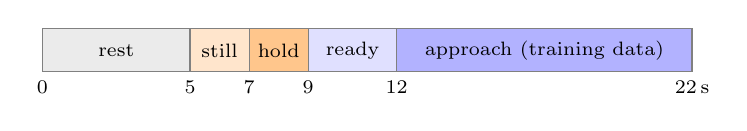
\begin{tikzpicture}[font=\scriptsize, x=0.375cm]
\foreach \a/\b/\t/\c in {0/5/rest/black!8, 5/7/still/orange!20, 7/9/hold/orange!45, 9/12/ready/blue!12, 12/22/approach (training data)/blue!30}
  {\fill[\c] (\a,0) rectangle (\b,0.55); \draw[black!50] (\a,0) rectangle (\b,0.55); \node at ({(\a+\b)/2},0.27) {\t};}
\foreach \x/\l in {0/0, 5/5, 7/7, 9/9, 12/12, 22/22\,s} \node[below] at (\x,0) {\l};
\end{tikzpicture}
\caption{HRA\_A100 take cycle: rest, jaw tip still on the taped cross, recording starts with a 2\,s origin hold, ready, 10\,s approach. The origin hold places the HandUMI jaw tip on the same taped cross that the robot jaw tip touched
during calibration.}
\label{p2:fig:protocol}
\end{figure}

\textbf{Task frame G.} The robot's right jaw tip touched three points on the tape line (far, centre, near); they are collinear
to within 0.38\mm over a 60.4\mm baseline and agree in height within 2\mm. G has its origin at the cross centre, $x$ along the
tape towards the human side and $z$ along base $z$: origin $(59.0, -74.9, 6.2)$\mm in the robot base, heading
47.09\textdegree. With the 35\mm plate the table is at $z=-27.1$\mm.

\textbf{Scale and orientation at the origin.} During the hold the fingertip is on the plate, so the first MASt3R keyframe's
pointmap contains the table plane at a known distance from the camera. Fitting up to three planes by RANSAC (excluding the
finger) and taking the largest one parallel to the plate gives a second scale source; against cube PnP on 40 takes its ratio
has a median of 0.999 and a per-episode error of p50 8\%, p90 37\%. Each episode uses cube PnP where it is valid and the
origin plane otherwise (35 and 72 of 107); the IMU is not used. The origin yaw is measured per episode by matching the table
around the cross (error p50 0.21\textdegree, p90 1.17\textdegree); assuming a mean yaw instead had produced false rejections
and a 57\mm endpoint-height spread (35\mm with measured yaw). The hold itself repeats to 14\mm (p50; p90 37\mm) and
6.2\textdegree{} (p50), with the camera pitched 63.7\textdegree{} down.

\textbf{Start-anchored versus origin-anchored state.} On 93 takes (82 train, 11 validation; the excluded 14 are the old
session, 7 takes in which the hand moved over 20\mm during the hold, and one physics failure) we trained two otherwise identical
models: A anchors the state at the hand pose at ``go'', B at a fixed origin frame F (the cross, with the tape heading and the
median hold pitch). Both use robot-TCP labels and the robot-camera rendering. Their held-out losses are close and both are
lowest at the first checkpoint (Table~\ref{p2:tab:val}, Fig.~\ref{p2:fig:val}b): A 0.124 and B 0.132 at 5k, rising to 0.224 (A, 50k)
and 0.190 (B, 45k). With 82 training takes, both models overfit from 5k steps. Neither anchoring is better on this measure.

\begin{figure*}[t]
\centering
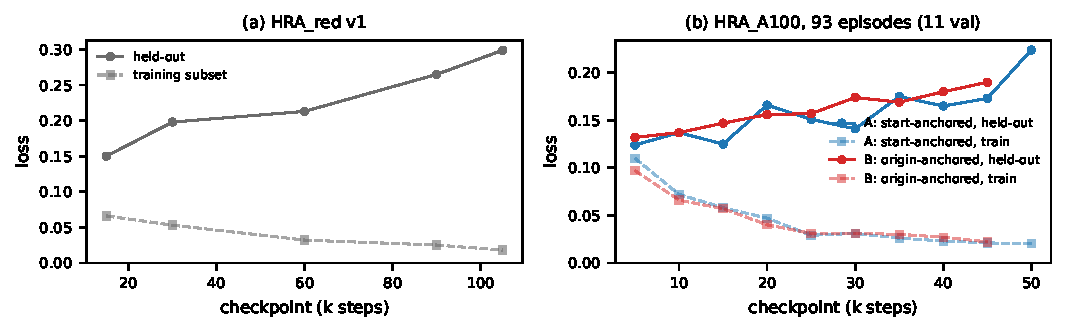
\includegraphics[width=0.8\textwidth]{../figures/fig9_hra_val.pdf}
\caption{Held-out (solid) and training-subset (dashed) loss by checkpoint. (a) HRA\_red v1, 15 validation takes. (b) HRA\_A100,
start-anchored (A) and origin-anchored (B) state, 11 validation takes. All runs overfit from the earliest checkpoint.}
\label{p2:fig:val}
\end{figure*}

\textbf{Table-aware conversion.} Expressing human motion in G and starting it from a robot start pose can push the fingertip
into the table. The conversion therefore re-anchors the start to the robot start pose with a weight that decays to zero over the
take, so the human endpoint near the cube is kept, and solves a small quadratic program per take with a hard floor at the
table plus 5\mm and a preferred clearance of 12\mm; an endpoint may be lifted by at most 30\mm. Table~\ref{p2:tab:ct} shows the
variants. CT4 decays position, height and rotation on separate schedules; CT5 adds measured origin yaw, the corrected IMU
gravity, absolute state in G and an origin-hold gate (hold within 10\mm of the origin); CT6 moves the robot start 6\,cm back and
4\,cm down. CT5 and CT6 keep 86 takes with fingertip clearance p50 12.6\mm and minimum 7.6\mm; most rejections are the old
session or takes whose origin yaw could not be measured.

\begin{table}[t]
\centering\footnotesize\setlength{\tabcolsep}{3pt}
\caption{Table-aware conversions of HRA\_A100. Accepted = PASS + PASS-CORRECTED. Clearance: fingertip above the table after
correction, accepted takes.}
\label{p2:tab:ct}
\resizebox{\columnwidth}{!}{\begin{tabular}{@{}lcccc@{}}
\toprule
Variant & Takes & Accepted & Main rejections & Clearance p50 / min \\
\midrule
C (mean yaw) & 107 & 81 & lift $>$30\,mm 10, old 7 & 19.5 / 7.0\mm \\
CT4 (per-axis decay) & 107 & 87 & lift 10, old 7 & 20.6 / 7.9\mm \\
CT5 (yaw, G, hold gate) & 107 & 86 & yaw not measured 9, old 7 & 12.6 / 7.6\mm \\
CT6 (start back/down) & 107 & 86 & as CT5 & 12.6 / 7.6\mm \\
CT7 (low start, +27) & 134 & 90 & IK 19, yaw 11, old 7 & 12.4 / 7.6\mm \\
\bottomrule
\end{tabular}}
\end{table}

\textbf{Start pose.} Where the robot starts matters for both views and reachability. We compared ten candidate start poses
derived from the median and medoid of the human ``go'' poses in G, moved back, right and down. The operator preferred the
lowest (pose 08, TCP $(273, -168, 116)$\mm, joint margin 9.1\textdegree). On 7 October 27 further takes were recorded with a
lower human start (origin to ``go'' about 89\mm instead of about 247\mm); from pose 08 only 5 of them pass, so they were dropped,
and the current run (CT7-old, 85 takes from 6 October, start 08, 100k-step schedule) uses only the 6 October data. CT5 and CT6
runs were stopped after 7k and 3k steps while settings changed; there is no validation split for CT6 and CT7.

\section{Deployment Settings That Mattered}\label{p2:sec:deploy}
\textbf{Chunk execution.} The interface blends successive 16-step chunks. With an exponential blend of 0.25, no cross-fade, no
smoothing and a minimum of one executed row per chunk, motion was acceptable; with the code defaults (0.35, 4 rows, 3\textdegree,
6 rows), which a restart of the interface silently restored on 7 October, the operator reported that ``inference quality had
dropped a lot'' until the values were restored. Inference quality on the robot therefore depends on settings that are not
part of the checkpoint; the loader now restores them.

\textbf{Tool-frame convention.} Models trained on robot-TCP labels (v2, A100) must run with zero camera pitch and zero
camera--TCP offset; the 33.1\textdegree{} pitch and offset of Sec.~\ref{p2:sec:robotcal} apply only to v1. Anchored models must be
served with the same anchor file (F for B, G for CT5--CT7).

\textbf{Cube-size stop.} On 7 October the operator observed the arm pushing the cube instead of stopping. Every 0.1\,s the
interface now measures the red cube's apparent size ($\sqrt{\text{area}}$ in pixels on the raw 640$\times$480 wrist frame) and
stops when two readings exceed a threshold (170--250\,px were used); in follow mode it resumes when the cube shrinks below 85\%
of the threshold. A cube-size stop means the cube looks large in the wrist view; it is a proximity proxy, not verified contact.
The wrist image was also zoomed 1.5$\times$ because the cube looked smaller than in training at the same position.

\textbf{Guards.} During v1 the interface stopped a run after 450\mm net travel, 80\mm between inferences, a still period, or
an output above 250\mm or 60\textdegree; a 6\,s time limit ended runs after 1--4 cycles and was removed. For A100 models all
numeric guards are off and the left arm and jaws stay locked.

\section{Robot Observations}\label{p2:sec:robot}
The interface's planned-execution log records 192 sessions on 6 and 7 October. On 6 October, 65 sessions (v1 checkpoints, the
chunk-setting tuning above) were all stopped by the operator except one, which the interface closed when a planned row jumped by
90.9\textdegree. On 7 October, 127 sessions ran: B 45k (3), A 50k (6) and CT5 5k (4), then B 50k with the 1.5$\times$ zoom (114
sessions, many of them follow-mode resumes); 69 of the 127 ended on the cube-size stop and 58 were stopped by the operator.
The log has no outcome field and the trial logger was not used, so we cannot say how many approaches reached the cube, and we
report no success rate. The cube appears orange in the fisheye-rendered training images and red on the robot camera, a colour
gap we have not corrected.

\section{Corrections}\label{p2:sec:corr}
Several of our own intermediate readings were wrong, each found by an independent check: the robot start tilt was 25\textdegree,
not 3\textdegree; the robot's wrist view is about 1.32$\times$ magnified and 11\textdegree{} lower than the human's, not
2.5$\times$; ``labels drive the tip 5\,cm into the table'' was the TCP--tip offset; the table height moved from $-54.3$ to
$-5.9$ to $-27.1$\mm as the contact model was fixed; IMU tilt statistics were off by up to 18\textdegree; and a mean origin yaw
caused false rejections. We list them because the same errors are easy to make in any human-to-robot calibration.

\section{Lessons}\label{p2:sec:lessons}
(i) \emph{Every scale source has a regime in which it fails silently}: the IMU on slow motion, cube PnP on oblique single-face
views, the origin plane on a few takes (p90 error 37\%); a second independent source is needed to see the failure.
(ii) \emph{A shared physical origin is cheaper than post-hoc registration}: linking 166 takes after the fact through a head
camera reached 64 takes with centimetre errors, while a taped cross touched by both the robot and the human gives a common
frame with sub-millimetre line fit. (iii) \emph{The TCP of the IK stack is a convention, not the fingertip}; contact
reasoning needs the fingertip geometry. (iv) \emph{Small single-task sets overfit at once}: with 80--150 takes, held-out loss
is lowest at the first checkpoint (5k or 15k), so the early checkpoints are the ones to test on the robot. (v) \emph{Execution
settings are part of the policy}: blend and smoothing parameters that live in the interface changed robot behaviour more than
a change of checkpoint, and must be recorded with every run.

\section{Limitations and Next Steps}\label{p2:sec:lim}
We have no success rate and no controlled comparison of datasets on the robot: runs were exploratory, settings changed between
them, and outcomes were not logged. The A100 data come from one operator, one scene and two days; the held-out sets are 11--15
takes. The cube colour differs between the rendered training images and the robot camera. The approach data teach a direction
towards one red cube; they make no claim about colour grounding. Next: log every robot trial (checkpoint, start pose, cube
position, reached yes/no, stop reason) with fixed execution settings; test early checkpoints (5k--15k) of A, B and CT7 from
the same start poses and cube positions; collect more A100 takes from the chosen start; correct the colour of the rendered
wrist images; and then use the approach prior as the first segment of the stacking policy of Part I.

\section{Conclusion}
For a single-arm approach, egocentric human data can be brought into the robot's frame with sub-centimetre consistency, but
only after replacing the IMU scale with object- and plane-based scale, calibrating the robot wrist camera, and anchoring every
take at a physical origin shared with the robot. Models trained on 80--150 such takes overfit quickly, and on the robot they move
towards the cube from nearby starts; with no logged outcomes, how often they reach it is still open.
\reportpart{Methods and Pipeline}{How each stage works (companion to Parts I and II)}{part:m}
\partabstract{This document describes, at the level of algorithms, parameters and gates, every stage we used to turn egocentric human
demonstrations into robot policies: the hand-worn recording rig and collection protocols, sensor and robot calibration,
synchronisation and export, monocular wrist-pose recovery and the three metric-scale sources (IMU, a cube of known size and a
table plane), two generations of conversion into robot training data (joint-space retargeting and a Cartesian action contract),
the single-arm variant with a shared task frame, the X-VLA model and its training recipes, the offline and diagnostic
evaluations, and deployment on the robot. File names refer to the repository unless stated otherwise. The last section lists
inconsistencies we found in our own code while writing it.}
\section{Overview}
Fig.~\ref{m:fig:overview} shows the stages. Each stage writes its output with a manifest and is followed by a gate that either
accepts a unit (episode, segment, row or take) or rejects it with a reason; the reports count what each gate removes. Two
conversions share the front end: generation~1 (Gen-1) retargets human wrist poses to robot joint trajectories, and generation~2
(Gen-2) expresses them in the same relative Cartesian action space as our robot teleoperation data. The single-arm approach data
(Part II) is a Gen-2 variant with masked dimensions and a physical origin shared with the robot.

\begin{figure*}[t]
\centering
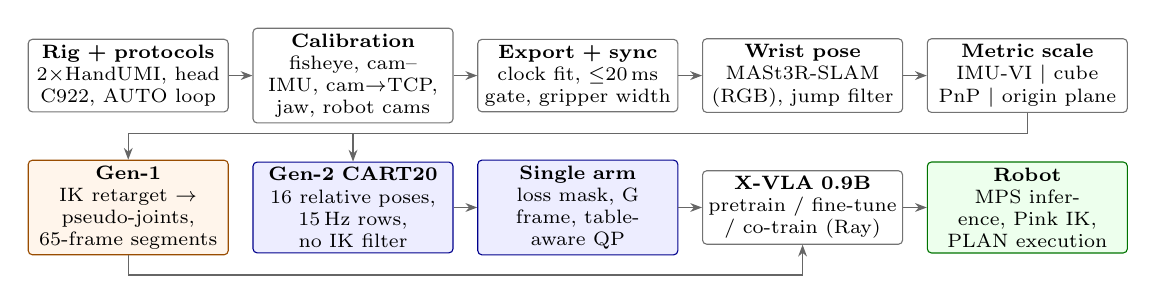
\begin{tikzpicture}[font=\scriptsize, node distance=3mm and 3mm,
  box/.style={draw=black!55, rounded corners=1.5pt, align=center, inner sep=2pt, minimum height=9mm, text width=24mm, fill=white},
  g1/.style={box, fill=orange!8, draw=orange!60!black}, g2/.style={box, fill=blue!7, draw=blue!55!black},
  dep/.style={box, fill=green!7, draw=green!45!black}, arr/.style={-{Stealth[length=1.5mm]}, draw=black!60}]
\node[box] (rig) {\textbf{Rig + protocols}\\2$\times$HandUMI, head C922, AUTO loop};
\node[box, right=of rig] (cal) {\textbf{Calibration}\\fisheye, cam--IMU, cam$\to$TCP, jaw, robot cams};
\node[box, right=of cal] (exp) {\textbf{Export + sync}\\clock fit, $\le$20\,ms gate, gripper width};
\node[box, right=of exp] (pose) {\textbf{Wrist pose}\\MASt3R-SLAM (RGB), jump filter};
\node[box, right=of pose] (scale) {\textbf{Metric scale}\\IMU-VI $\mid$ cube PnP $\mid$ origin plane};
\node[g1, below=6mm of rig] (g1) {\textbf{Gen-1}\\IK retarget $\to$ pseudo-joints, 65-frame segments};
\node[g2, right=of g1] (g2) {\textbf{Gen-2 CART20}\\16 relative poses, 15\,Hz rows, no IK filter};
\node[g2, right=of g2] (hra) {\textbf{Single arm}\\loss mask, G frame, table-aware QP};
\node[box, right=of hra] (train) {\textbf{X-VLA 0.9B}\\pretrain / fine-tune / co-train (Ray)};
\node[dep, right=of train] (dep) {\textbf{Robot}\\MPS inference, Pink IK, PLAN execution};
\draw[arr] (rig)--(cal); \draw[arr] (cal)--(exp); \draw[arr] (exp)--(pose); \draw[arr] (pose)--(scale);
\draw[arr] (scale.south) |- ++(0,-2.6mm) -| (g1.north); \draw[arr] (scale.south) |- ++(0,-2.6mm) -| (g2.north);
\draw[arr] (g2)--(hra); \draw[arr] (hra)--(train); \draw[arr] (train)--(dep);
\draw[arr] (g1.south) |- ++(0,-2.5mm) -| (train.south);
\end{tikzpicture}
\caption{Pipeline overview. Orange: generation 1 (joint space); blue: generation 2 (Cartesian) and its single-arm variant; green:
deployment. Every arrow is followed by a gate with a logged reason.}
\label{m:fig:overview}
\end{figure*}

\section{Recording Rig and Collection Protocols}\label{m:sec:rig}
\textbf{Rig} (\code{collection/configs/handumi/hardware_handumi_v1.yaml}). HandUMI~\cite{handumi_hw} is an open-source hand-worn
UMI variant designed and published by BrikHMP18, not by us (\url{https://github.com/murobotics-ai/handumi-hw}, formerly
\texttt{robonet-ai}); we use its body, linkage and
servo-encoder jaw from commit \texttt{e58de33} but not its VR tracking (Part~I, Sec.~III). Each unit carries an Arducam fisheye UVC
camera (1920$\times$1080, 30\,fps, MJPG), an ICM-42688-P IMU on a Teensy~4.1 (nominal 200\,Hz; measured 201.6 and 197.9\,Hz
because each board has its own oscillator) and a Feetech STS3215 servo used as a jaw encoder (4096 ticks/rev, polled at
100\,Hz). Both wrist cameras report the same USB serial, so they are matched by product name. A fixed Logitech C922
(640$\times$480, 30\,fps, autofocus off) records the table; an RGB-D camera was dropped because it disrupted the wrist streams.

\textbf{Recording} (\code{collector/recorder.py}). An episode directory holds one MP4 per camera, \code{sensors.mcap},
\code{events.json} and \code{episode_meta.json}; it is renamed from \code{.incomplete} to \code{.complete} only when closed.
MCAP JSON channels carry IMU samples (device and host timestamps, accelerometer, gyro), gripper samples (unwrapped and wrapped
ticks, normalized value), per-frame metadata (frame index, capture time, skipped frames), events and clock anchors. All streams
are stamped with the host monotonic clock: the IMU at host receive time, the gripper at the midpoint of the serial
transaction, frames at capture.

\textbf{AUTO loop} (\code{collector/autoloop.py}). A state machine RESET $\to$ ARMING $\to$ HOLD $\to$ (PREP) $\to$ EPISODE
$\to$ STOP drives each take with spoken cues. ARMING waits for stillness: in 0.25\,s windows the mean gyro magnitude must be
below 6\textdegree/s, the accelerometer-magnitude standard deviation below 0.35\,m/s$^2$, the largest sample gap below 25\,ms and
the window at least 60\% filled, for a continuous run of 1\,s. A hold after recording starts gives the visual--inertial
initialisation window. A take that passes preliminary QA is kept automatically; a failure pauses the loop.
\begin{itemize}
\item \emph{Stacking}: 20\,s takes, 10\,s reset, 3\,s hold; the next order is the one with the fewest kept takes
(\code{episode_manager.next_order}), so orders are balanced rather than randomized.
\item \emph{Robot-like} (\code{robot_like_v1}): 30\,s takes with live feedback. Wrist angular speed and angular acceleration
on a 15\,Hz grid are compared with the 95th percentiles of robot teleoperation data (0.996\,rad/s, 4.413\,rad/s$^2$); a take is
sent to review if more than 10\% of ticks exceed them or fewer than two grasps occur.
\item \emph{Approach} (HRA\_red): right hand only, 10\,s takes, 5\,s reset, gripper checks off.
\item \emph{Approach with origin} (HRA\_A100): 5\,s rest; 2\,s still with the jaw tip on a taped cross; recording starts with a
further 2\,s origin hold (event \code{go_cue}); a 3\,s ``ready'' move to a robot-like start; at ``go'' a 10\,s approach. The
right wrist also records a robot-camera-like view.
\end{itemize}

\textbf{Collection QA} (\code{collector/integrity.py}). A take goes to review on device or recorder error events, an empty
stream, or a frame rate below 25\,fps; it is rejected if the gripper is sampled below 20\,Hz, frozen, outside its calibrated
span by more than 300 ticks, or travels less than 5\% of its range. Validation decodes every video to its metadata frame count
and checks that frame indices are contiguous and capture times strictly increasing.

\section{Calibration}\label{m:sec:cal}
\textbf{Wrist cameras.} Kannala--Brandt (equidistant) fisheye models at full resolution, fitted with Kalibr on an 8$\times$5
checkerboard of 25\mm squares (left $f_x{=}788.9$\,px). \textbf{Camera--IMU.} Kalibr~\cite{furgale2013kalibr} extrinsics and time
offsets per hand. \textbf{Camera to TCP} (\code{calibration/camera_tcp/handumi_camera_tcp_v2.yaml}). The TCP is the pinch
centre with $x$ along the approach direction, $y$ along jaw closing and $z = x\times y$. The rotation is a fixed axis permutation
($x_\text{TCP}=z_\text{cam}$, $y_\text{TCP}=-x_\text{cam}$, $z_\text{TCP}=-y_\text{cam}$); the translation comes from caliper
measurements (95\mm forward, 95\mm down) rotated by the camera pitch measured from IMU gravity (20.7\textdegree), giving
$t=(0, 55.3, 122.5)$\mm, consistent to about 1\mm with a cube-based fit. It was measured on one unit and applied to both.
\textbf{Head camera.} A provisional plumb-bob model ($f=677.7$\,px).

\textbf{Robot side} (Part II). The robot's fixed camera is calibrated on the same checkerboard ($f=728.7$\,px, RMS 1.05\,px); the
right jaw tip touches four inner corners, the forward-kinematics (FK) TCP positions and the board pose from PnP give
$T_\text{base,board}$ by Kabsch alignment, and $T_\text{base,cam}=T_\text{base,board}T_\text{cam,board}^{-1}$. The robot
wrist camera is calibrated from 13 board views (intrinsics with fixed aspect, no tangential distortion, RMS 0.16\,px) and its
hand-eye transform is solved with the Tsai, Park, Horaud and Daniilidis methods~\cite{tsai1989handeye}; Park's solution is used.
Physical contact is modelled by the URDF fingertip box (70--80\mm behind the IK TCP along $x$, $\pm$19.6\mm in $z$), whose
lowest corner counts as the contact point.

\section{Export and Synchronisation}\label{m:sec:export}
\textbf{Clock alignment} (\code{pose/timing.py}). IMU device time is mapped to host time by a least-squares slope with the
intercept re-anchored at the 5th percentile of the residuals, because USB latency only ever adds delay; the camera--IMU time
offset from calibration is then applied. Cameras free-run at slightly different rates (30.003--30.026\,Hz), so frames are paired
by nearest capture time rather than by a constant offset.

\textbf{Export} (\code{pipeline/export/umi_export_orbslam.py}). Each wrist is written as a 960$\times$540 video (intrinsics
halved), an IMU file in GoPro-telemetry layout with 50\,ms of IMU before the first frame, and a camera settings file; frames and
capture times come from a single decoding pass so they cannot drift apart.

\textbf{Synchronisation gate} (\code{pipeline/census/c8_census_pre.py}, \code{c8_phase3.py}). The left wrist is the master
clock; the right wrist and the head camera are matched by nearest capture time. A row is valid if both wrist poses are valid and
both matches are within 20\,ms ($\Delta t_R<20$\,ms and $\Delta t_H<20$\,ms). An episode passes if it contains at
least one run of 65 consecutive valid rows.

\textbf{Gripper width} (\code{pipeline/grip/}). Each frame takes the nearest gripper sample. Because the recorded normalized value
was unreliable (the open end lay beyond the mechanical stop and the left direction flipped between sessions), Gen-1 recomputes
the width from raw ticks: direction from the open/closed tick pair, a closed anchor from per-episode closed extremes, the open end
at the closed anchor plus the device span (1136.6 / 1248.2 ticks), and width $= \mathrm{clip}(f,0,1)\times 67.5$\mm. Gen-2 uses a
later caliper calibration (gcal1): piecewise-linear knots at 0/20/40/60/80\mm, normalized as $g=\mathrm{clip}(w/80\,\text{mm},0,1)$,
0 = closed.

\section{Wrist Pose and Metric Scale}\label{m:sec:pose}
\textbf{Monocular pose} (\code{pipeline/mast3r_pose/run_perframe.py}). MASt3R-SLAM~\cite{murai2025mast3rslam} (official
code, pinned commit; the only patch is a build fix) runs on the RGB wrist video undistorted to a pinhole view, single-threaded,
every frame, fixed seed. After global optimisation every frame is re-expressed on its final keyframe:
\begin{equation}
T_{WC}(f) = T_{WK}^{\text{final}}(k)\,T_{WK}^{\text{track}}(k)^{-1}\,T_{WC}^{\text{track}}(f),
\end{equation}
a Sim(3) chain; frames tracked during relocalisation are invalid unless they later became keyframes. The UMI approach of one
ORB-SLAM3 map per scene~\cite{chi2024umi} was replaced because it failed to relocalise after scene changes.

\textbf{IMU visual--inertial scale} (\code{cp6_scale.py:imu_vi}). The SLAM trajectory is metric up to a per-episode scale $s$.
With $R_{wb}=R_{wc}R_{cb}$, accelerometer samples $f_b$ box-averaged around each frame, the camera acceleration $a_\text{cam}$ and
the lever-arm acceleration $a_\text{lever}$ obtained as Savitzky--Golay second derivatives (order 3, window $W$) of the SLAM camera
position and of $R_{wc}t_{cb}$, each frame contributes three rows of
\begin{equation}
R_{wb}\,f_b - a_\text{lever} = s\,a_\text{cam} - g\;\;(+\,R_{wb}b_a),
\end{equation}
solved for $s$ and $g\in\mathbb{R}^3$ by Huber-weighted iteratively reweighted least squares (10 iterations, $\sigma=1.4826\,$MAD)
over the longest valid run. Both sides pass the same filter, so they share the band limit, and nothing is integrated twice.
$W=15$ without bias was selected on a fit split of the marker benchmark. A scale is valid if $s>0$, $|g|\in[8.81,10.81]$\,m/s$^2$
and $s$ lies within 0.1$\times$ the smallest and 10$\times$ the largest benchmark scale. Metric TCP poses are $T_\text{tcp}=
(T_{WC}\text{ with translation}\times s)\,X_\text{cam,tcp}$.

\textbf{Pose benchmark.} 14 demonstrations (28 hand tracks; 9 for fitting, 5 held out) with four 80\mm ArUco markers in view.
Marker poses are solved with IPPE on undistorted points; markers more than 20\textdegree{} from the consensus are rejected.
Ground-truth scale is the median ratio of marker to SLAM displacement over frame pairs ten frames apart in which a marker moved
more than 30\mm. Reported: coverage, scale error, rotation error, a UMI-style 16-step relative position error and the rate of
direction reversals.

\textbf{Camera--IMU consistency.} Sessions whose gyro and SLAM angular velocities disagree (median cosine near 0 against
0.92--0.98 elsewhere) are quarantined. For the approach data, the exported camera--IMU rotation of the right wrist was corrected by
about 18\textdegree{} about the camera $x$ axis after comparison with the cube and table geometry.

\textbf{Pose-jump filter} (\code{cart20/ego_cart20/preprocessing/pose_filter.py}). MASt3R-SLAM occasionally moves the camera by
centimetres within one frame without a loss flag. A raw step is flagged when the displacement over one 66.7\,ms row exceeds 100\mm{}
or 45\textdegree{} and the jump lies in that step, or when a step above 50\mm is isolated between steps slower than 0.3\,m/s.
Flags within 5 samples form one event. If the pose returns (within $\max(30\,\text{mm}, 0.3\times\text{step})$ and 45\textdegree)
the event is a spike and only its samples are invalidated; otherwise it is one-way and the rest of that arm's track is
invalidated, because a start-anchored state would be wrong from then on.

\textbf{Cube PnP scale} (\code{cart20/ego_cart20/cube_pnp.py}; Part II). For slow motions the IMU fit is unobservable. The red
cube (edge 38\mm) is segmented in HSV, its convex hull reduced to six (or four) vertices whose corners are sharpened by line fits
to the middle of each side, and fitted by PnP with two- and three-face silhouette models (with a visibility check: the faces the
camera lies in front of must equal the model's visible faces) or, within 35\textdegree{} of head-on, a single-face IPPE model with
the centre placed half an edge behind the face. Since the cube is static, its centre $c_i=p_i + k\,R_i t_i$ must be constant, which
gives the inverse scale in closed form,
\begin{equation}
k = -\frac{\sum_i (p_i-\bar p)\cdot(u_i-\bar u)}{\sum_i\lVert u_i-\bar u\rVert^2},\qquad u_i=R_i t_i,\quad s=1/k,
\end{equation}
with MAD trimming and 200 bootstrap resamples. A take needs at least 10 PnP frames, a bootstrap spread of at most 10\% and a
centre residual of at most 2\,cm.

\textbf{Origin-plane scale} (Part II, HRA\_A100). During the origin hold the fingertip touches the plate, so the first SLAM keyframe
sees the table at a known distance. Excluding the finger region and low-confidence points, up to three planes are fitted by RANSAC
(400 iterations, threshold 0.4\% of the median depth) and the largest one parallel to the first is taken as the table; then
$s=|n\cdot t_\text{tip}|/(s_0\,|d|)$ with $t_\text{tip}$ the fingertip in camera coordinates and $s_0$ the keyframe's Sim(3) scale.
Cube PnP is used when valid, otherwise the plane.

\section{Generation 1: Joint-Space Retargeting}\label{m:sec:gen1}
\textbf{Segments and gates} (\code{c8_phase3.py}). Valid rows are cut into non-overlapping 65-frame blocks (2.17\,s). Per arm, a
segment must have a valid metric scale (B), keep at least 95\% of rows inside the robot workspace (C; a target is inside if its
nearest neighbour among 6{,}000 robot teleoperation TCP poses is within 50\mm{} and the smallest of the 50 nearest orientation
differences is below 20\textdegree), solve IK on every row (D) and yield finite joints (E). A segment is bimanual if both arms
pass.

\textbf{Retargeting} (\code{pipeline/pseudo_joint/pseudo_joint_pipeline.py}). Human motion is taken relative to the segment start
and mapped into the robot dataset's TCP frame, $\text{rel}=F^{-1}T_{0}^{-1}T_{t}F$ with $F=R_x(180^\circ)$, and placed at a fixed
robot anchor posture (the median active posture of robot teleoperation data): $T_\text{tgt}=\mathrm{FK}(q_\text{anchor})\,C^{-1}\,
\text{rel}\,C$, $C=R_y(90^\circ)$. A least-squares IK (pose cost with orientation weight 20, a rest term towards the previous
solution, joint-limit constraints, at most 10 iterations, joint step at most 0.35\,rad) is seeded from the previous row; rows are
labelled LIMIT, DQ\_FAIL ($>$1\,rad), BRANCH\_SWITCH ($>$0.3\,rad while the target barely moves), NOT\_CONVERGED ($>$15\mm{} or
$>$5\textdegree) or OK.

\textbf{Dataset and targets} (\code{pipeline/dataset/}, \code{training/humanik_delta.py}). One LeRobot episode per segment: three
640$\times$480 views, a 14-D state (six joint angles and a gripper value per arm) and the target TCP poses. The policy predicts 30
cumulative joint displacements $a_i=q_{t+5+i}-q_t$ (a 5-frame lead) and an absolute binary gripper. Two auxiliary losses tie joint
space to the measured motion: (C) the relative TCP translation $\mathrm{trans}(T_\text{tgt}(t)^{-1}T_\text{tgt}(t{+}5{+}i))\times10$
in spare action dimensions, and (D) an FK consistency term,
\begin{equation}
\mathcal{L}=\mathcal{L}_{\Delta q}+\mathcal{L}_\text{grip}+2.0\,\mathcal{L}_C+20\,\lVert \mathrm{FK}(q_t+\hat a)-p_\text{tgt}\rVert^2 .
\end{equation}
The split draws 10\% of source episodes with a fixed seed; no episode spans both sides.

\textbf{Retargeting v2} (\code{pipeline/retarget_v2/}). The single anchor made every segment start from one posture. v2 uses only
30 robot episodes for calibration (evaluating on 120 others). A seed bank of $2^{17}$ Sobol samples of both arms' joints is filtered
by workspace, table floor, manipulability (smallest singular value of the position Jacobian) and inter-arm clearance $\ge$75\mm{}
(exact segment-to-segment distances between 9 link segments per arm), then de-duplicated (1{,}195 seeds). Variant K rolls out the
best 8 seeds and scores $S=\overline{e_\text{pos}}/15+\overline{e_\text{rot}}/5+\overline{|\Delta q|}/0.6+0.5\,\overline{|\Delta^2q|}/0.6$;
Kr adds the posture distance to robot data; TR retrieves the 64 nearest robot trajectory windows by a 96-D relative-motion
feature, keeps feasible ones and seeds IK with $q_\text{last}+\Delta q_\text{ref}$. A hybrid keeps TR when feasible, otherwise Kr.

\section{Generation 2: The Cartesian Contract (CART20)}\label{m:sec:gen2}
\textbf{Contract} (\code{cart20/ego_cart20/config.py}). Rows at 15\,Hz; offsets $\Delta=3/59.94$\,s $=50.05$\,ms, the robot data's
step. For row time $t$ and each arm,
\begin{equation}
A_k = T(t)^{-1}\,T(t+k\Delta),\qquad k=1,\dots,16 ,
\end{equation}
current-anchored (not sequential), interpolated on the raw 30\,Hz track (linear position, SLERP rotation, linear gripper; only
between valid samples at most 50\,ms apart; no extrapolation). Each arm contributes [position 3 $\mid$ 6-D rotation (the first two
rows of $R$, decoded by Gram--Schmidt) $\mid$ gripper], so two arms give 20 dimensions; the model's 32-D action is padded with 12
dimensions that are exactly zero. The state is each arm's pose relative to its own task-start pose, $T(t_0)^{-1}T(t)$, plus both
grippers (there is no shared left--right SLAM frame).

\textbf{Conversion} (\code{convert.py}). Pose-jump filter; per-arm interpolation tracks; task start at the first instant both arms
are valid; nearest head frame within 20\,ms. A row is a training row only if both arms are valid at $t$, all 16 targets are valid
and a head frame exists; there is no padding. No workspace or IK selection is applied.

\textbf{Validation} (\code{validation/}, \code{tests/}). Shapes, zero padding, finite values, $g\in[0,1]$, orthonormal rotations with
determinant $+1$, identity start state, disjoint splits, no target beyond the last valid row, and median translation increasing with
$k$; eleven synthetic tests pin the contract.

\textbf{Robot-like wrist rendering} (\code{scripts/export_lerobot_robotized.py}). To narrow the visual gap, a fisheye frame is
re-rendered as a virtual pinhole camera with the same orientation (so labels stay valid): horizontal field of view drawn from
62--70\textdegree, principal point shifted 75--125\,px down so the jaws sit low as on the robot, then downscaled, blurred
($\sigma$ 0.4--1.0), JPEG-compressed (quality 55--85) and photometrically jittered, with a per-frame seed. ROBOT100 applies it to
every frame. The single-arm robotcam v2 rendering (Sec.~\ref{m:sec:hra}) instead uses the measured robot camera.

\textbf{Export.} LeRobot v3 at 15\,fps, three 224$\times$224 views, statistics recomputed (padding dimensions mean 0, std 1); the
joint fields are NaN on purpose so that any joint-space loss fails loudly.

\section{Single-Arm Variant and Shared Task Frame}\label{m:sec:hra}
\textbf{Right-only contract} (\code{right_only.py}). The tensor layout is unchanged: the left state is the identity pose with
gripper 0, the left action is zero motion, and a per-episode 20-D loss mask supervises only the right arm's position and rotation
(9 dimensions; the gripper was static and masked).

\textbf{Robot-camera rendering} (robotcam v2). For each robot-camera pixel, the ray from the measured robot intrinsics is projected
into the fisheye model and resampled (rays outside the fisheye view are black), with small focal and principal-point jitter and the
same degradation chain. Labels are moved from the UMI TCP to the robot TCP through the hand-eye transform, $T_\text{robot}=T_\text{UMI}M^{-1}$.

\textbf{Task frame G.} Three robot jaw-tip touches on the taped line give the origin (cross centre), $x$ along the tape and $z$ along
base $z$. At the human side, the origin pose is the median position and mean rotation over the hold; its yaw is measured per take by
matching table features around the cross (ORB, ratio test, PnP-RANSAC) against a reference take, with tilt from IMU gravity
(corrected extrinsic). The state is then the absolute pose in G and labels are $T_G = T_{\text{base},G}\,R(\text{yaw})\,
T_\text{origin}^{-1}T_\text{robot}$.

\textbf{Table-aware conversion.} The human trajectory is warped from its own start towards a chosen robot start pose $T_S$ with
smoothstep weights $\mathrm{sst}(x)=3x^2-2x^3$ over normalized time $s$: $w_{xy}=1-\mathrm{sst}((s-0.2)/0.6)$, $w_z=1-\mathrm{sst}(s/0.3)$,
$w_\text{rot}=1-\mathrm{sst}((s-0.1)/0.5)$, so the endpoint near the cube is the human's. A height correction $c$ is then solved
per take as a quadratic program,
\begin{equation}
\begin{aligned}
\min_c\;& \textstyle\sum c^2+50(\Delta c)^2+2000(\Delta^2 c)^2+60\,m\,(c-g)^2\\
\text{s.t.}\;& z_\text{tip}+c\ge z_\text{table}+5\,\text{mm},
\end{aligned}
\end{equation}
with $c_0=0$, the endpoint lift at most 30\mm{} and $g$ pulling low frames towards 12\mm{} clearance. The result is replayed through
IK (every second frame; error below 5\mm{} and 3\textdegree, joint margin above 2\textdegree). Takes are classed PASS (lift
$\le$20\mm), PASS-CORRECTED (20--30\mm), REVIEW, EXCLUDED or REJECT (IK success below 98\%, missing origin hold or yaw, hold moved
more than 10\mm, start below the floor); only the first two are exported.

\section{Model}\label{m:sec:model}
X-VLA~\cite{zheng2025xvla} through LeRobot~\cite{cadene2024lerobot}: a Florence-2~\cite{xiao2024florence2} vision-language encoder,
a 24-layer soft-prompted transformer (hidden 1024, 16 heads) and a flow-matching~\cite{lipman2023flow} action head; about 0.9B
parameters, all trainable. Inputs are three views resized with padding to 224$\times$224, the instruction (BART tokenizer) and the
proprioceptive state. \textbf{Soft prompts.} An embedding table of 30 domains $\times$ 32 tokens is appended to the sequence, and the
state/action projections are domain-specific linear layers; the domain id is set in the checkpoint's preprocessor. Reading the
public weights showed that only domains 10--17 had ever been trained; we use the unused domain 20 for our embodiment.
\textbf{Flow matching.} Training draws stratified $t$, forms $x_t=\varepsilon t+a(1-t)$ and regresses the clean action $a$
directly. Inference starts from $x_1\sim\mathcal N(0,I)$ and for $i=N\dots1$ sets $t=i/N$, $x_t=x_1 t+\hat a(1-t)$, $\hat a=f(x_t)$,
reusing $x_1$ (10 steps by default). \textbf{Widening for Gen-2.} The public head (20-D action and state) was widened to a 32-D
action and 20-D state: existing rows are copied exactly, new rows drawn from the base rows' scale, new biases zero, and the widened
model checked to reproduce the base for every domain.

\section{Training}\label{m:sec:train}
\textbf{Gen-1} (\code{training/train_bi.py}). The joint-displacement target and losses of Sec.~\ref{m:sec:gen1}, AdamW (learning
rate $10^{-4}$, the vision-language group at 0.1$\times$, weight decay $10^{-4}$, gradient clip 10), 1k warm-up and cosine decay to
$2.5\times10^{-6}$, batch 4, fp32 with TF32, 300k steps, a checkpoint every 10k. A 20-step smoke run must log finite losses and
active auxiliary terms first. The checkpoint selection rule (minimum geo score on validation) was fixed before training.

\textbf{Gen-2, REL-only} (\code{training/relonly/}). The loss is the MSE on action dimensions 0--19; the transformer is patched so that
dimensions 20--31 are zero at its input and output at every denoising step, in training and at inference. A preflight checks that the
loss ignores randomized padding targets, that padding predictions are exactly zero and that their decoder gradients vanish. 8-bit
AdamW (bitsandbytes) with a save shim, bf16 autocast with fp32 master weights, batch 8, seed 1000, warm-up 1k, cosine decay ending
exactly at the last step (the launcher refuses runs whose step count and decay differ, because LeRobot silently rescales the
schedule). Actions are mean/std-normalized, states not. \textbf{Loss mask} (single arm): masked targets are replaced by the detached
prediction before subtraction (avoiding NaN gradients) and the loss is normalized by the number of supervised elements.
\textbf{Fine-tuning} starts a fresh optimizer from the pretrained weights and uses the robot dataset's normalization statistics;
episode subsets (e.g.\ R30) are selected by index list. \textbf{Co-training} draws exactly four ego and four robot samples per batch.

\textbf{Operations.} Jobs are submitted to a Ray cluster and pinned to a GPU node (RTX~4090 or RTX~5090; their PyTorch versions
differ, so cross-node runs are not bit-identical). Launchers refuse to start on a busy GPU, a code-hash or domain-id mismatch, a
failed gripper-contract gate or low disk space, and a disk guard stops training before the node fills. A 60-step smoke run (with
save and resume) precedes each main run. An archiver copies every checkpoint to external storage with SHA-256 verification before
deleting it from the node, keeping optimizer state only at fixed intervals.

\section{Evaluation}\label{m:sec:eval}
\textbf{Gen-1 offline} (\code{evaluation/c8old_mac_eval.py}). On held-out episodes, seven start frames per segment (every 5 frames
in 0--30); one flow sample per start with a fixed seed. For horizons $k\in\{1,4,8,16,30\}$: TCP error $\lVert\mathrm{FK}(q_t+\hat
a_k)-p_k\rVert$ (median, p90), joint MAE, the MAE of a zero-motion predictor, and the cosine of predicted versus measured TCP
displacement. The geo score is the mean of median TCP errors over horizons; a collapse ratio compares prediction and target spread.
The moving subset requires at least 20\mm{} of TCP motion by $k{=}30$. \textbf{Prompt swap}: each sample is run with all six order
instructions under one seed and with the true instruction under two more seeds; instruction spread is compared with seed spread,
and the true instruction's error rank among the six with chance. \textbf{Paired bootstrap}: episode-level resampling (10k draws,
identical for both models) of the relative difference in geo score between two initializations.

\textbf{Gen-2 diagnostics} (\code{analysis/v3/}). Teacher-forced direction cosine on robot frames (predicted versus recorded
translation at $k$=4/8/16 for frames moving more than 10\mm), repeated under all left/right swaps and axis sign flips; an image/state
domain swap (ego or robot images combined with ego, robot or zero state); optical-flow versus pose-axis correlation of the wrist
videos (a convention check); and wrist-image sharpness as the variance of the Laplacian. \textbf{Training-loss comparisons}: losses
are parsed from logs (step = line index $\times$ log interval) and compared as window means and ratios. \textbf{Held-out loss}
(single arm): the training loss (masked) on all validation rows with two noise seeds and on a 2{,}000-row training subset.

\textbf{Claim verification} (\code{analysis/verify_claims.py}). Every number in the reports is recomputed from evidence files in the
repository at the printed precision, and required and retired strings are checked in the report sources and the README.

\section{Deployment on the Robot}\label{m:sec:deploy}
\textbf{Inference.} The policy runs on a Mac (Apple-silicon GPU, bf16) with 5 (bimanual) or 10 (single arm) denoising steps and the
REL-only zero patch. The three robot cameras are captured at 640$\times$480, optionally zoomed (right wrist, single arm), resized to
224$\times$224 and normalized as in training; in single-arm mode the left wrist image is black. \textbf{State} follows the training
contract: TCP poses from FK of the measured joints, with a fixed frame correction between the FK and dataset TCP conventions, relative
to an anchor taken at run start or to a fixed anchor file (G for the origin-anchored models). \textbf{Decoding}: absolute targets
$T_k=T_\text{now}A_k$ for $k=1..16$; the gripper value maps to a 0--45 command (robot raw 0 = closed, $-270$ = open), or the jaws are
held in single-arm mode.

\textbf{IK} (Pink~\cite{caron2024pink}). The URDF with locked fingers; the TCP is 70\mm{} along $x$ from the gripper link (identical to
the dataset TCP); per-arm frame tasks (position 1.0, orientation 0.5) and a light posture task, solved by quadratic programming from the
measured joints, with joint-limit margins and a per-waypoint joint-step limit. Profiles lock or free the wrist-yaw joint; other solvers
(numerical, learned, GPU-batched) can be switched at run time.

\textbf{Execution.} \emph{Step mode} executes a few waypoints of each chunk and waits until the arm settles. \emph{PLAN mode} keeps one
forward pass in flight and streams IK-solved rows (50.05\,ms apart) to the robot service, which plays them as 100\,Hz knots with
velocity feed-forward; rows still to be executed within the expected latency are reserved and only later rows are replaced. Seams
between chunks are handled by a joint-space exponential blend (\code{plan_ema}), an optional cross-fade, optional polynomial
smoothing and a minimum number of executed rows before the next forward pass; these values change behaviour visibly and are recorded
with each run. \emph{Real-time chunking} (optional): at each flow step the prediction is pulled towards the previous chunk's
not-yet-executed targets, $\hat x\leftarrow\hat x+t\,g_w\,J^\top(W\odot(Y-\hat x))$ with a guidance weight capped at 10 and $W$ decaying
over the first 8 steps~\cite{black2025rtc}.

\textbf{Robot service.} Two arm controllers in MIT impedance mode with an integral feed-forward term, a 100\,Hz control thread and an
acceleration-limited synchronized profile; raw joint limits are clipped, and a planned knot jumping more than 90\textdegree{} makes
the arm hold. \textbf{Safety and stops.} NaN predictions abort; in single-arm mode the left arm and jaws are always held; optional
travel, step and output guards; a \emph{cube-size stop} measures the red cube's apparent size ($\sqrt{\text{area}}$ in pixels of an
HSV mask on the raw wrist frame) every 0.1\,s and stops after two readings above a threshold, with an optional follow mode that
resumes when it shrinks below 85\% of the threshold. \textbf{Checkpoints} are pulled from the training node or the archive, verified
by SHA-256 and identity (run, dataset, domain), and loaded by restarting the interface. \textbf{Trial logging}: an operator form
records checkpoint, model type, robot data, instruction, layout, stack level 0--3, wrong colour, failure reason and the run's stop
reason; success is defined as level 3 with the right colours.

\section{Known Inconsistencies}\label{m:sec:issues}
Writing this down exposed the following, which we list rather than hide. (1) An inter-arm clearance check exists but is used only in
retargeting v2, not as a Gen-1 gate (an earlier README sentence said otherwise and was corrected). (2) In the Gen-1 target code a
binarized gripper label 1 means \emph{open}, although a comment says closed. (3) Three gripper calibrations are in use (Gen-1 ticks with
a 67.5\mm{} aperture, the gcal1 caliper knots for Gen-2, and the collector's open/closed files); each dataset names its own. (4) The
camera--IMU time offsets used by the exporter differ in sign and magnitude from the raw calibration output, and the step that converted
them is not recorded. (5) Two different right fisheye calibration versions are used by the exporter and by one viewer tool. (6) The IK
step thresholds are documented per 15\,Hz row but applied on 30\,fps rows. (7) In PLAN mode the bimanual path does not pass gripper
widths to the waypoint solver, so the jaws would likely stay closed; the single-arm runs, which hold the jaws, are unaffected.
(8) Several diagnostics were run from scripts outside the repository and their outputs are stored as captured logs, not re-run.
(9) Fitting scripts for the G frame, the fingertip box and the 18\textdegree{} camera--IMU correction are not in the repository; only
their outputs are.
\clearpage\renewcommand{\refname}{References}
\phantomsection\label{part:refs}
\begin{thebibliography}{99}\footnotesize
\bibitem{chi2024umi} C.~Chi, Z.~Xu, C.~Pan, E.~Cousineau, B.~Burchfiel, S.~Feng, R.~Tedrake, and S.~Song, ``Universal manipulation interface: In-the-wild robot teaching without in-the-wild robots,'' in \emph{RSS}, 2024.
\bibitem{wang2024dexcap} C.~Wang, H.~Shi, W.~Wang, R.~Zhang, L.~Fei-Fei, and C.~K. Liu, ``DexCap: Scalable and portable mocap data collection system for dexterous manipulation,'' in \emph{RSS}, 2024.
\bibitem{kareer2024egomimic} S.~Kareer \emph{et al.}, ``EgoMimic: Scaling imitation learning via egocentric video,'' \emph{arXiv:2410.24221}, 2024.
\bibitem{wang2023mimicplay} C.~Wang \emph{et al.}, ``MimicPlay: Long-horizon imitation learning by watching human play,'' in \emph{CoRL}, 2023.
\bibitem{grauman2022ego4d} K.~Grauman \emph{et al.}, ``Ego4D: Around the world in 3,000 hours of egocentric video,'' in \emph{CVPR}, 2022.
\bibitem{zhao2023act} T.~Z. Zhao, V.~Kumar, S.~Levine, and C.~Finn, ``Learning fine-grained bimanual manipulation with low-cost hardware,'' in \emph{RSS}, 2023.
\bibitem{chi2023diffusion} C.~Chi, S.~Feng, Y.~Du, Z.~Xu, E.~Cousineau, B.~Burchfiel, and S.~Song, ``Diffusion policy: Visuomotor policy learning via action diffusion,'' in \emph{RSS}, 2023.
\bibitem{kim2024openvla} M.~J. Kim \emph{et al.}, ``OpenVLA: An open-source vision-language-action model,'' in \emph{CoRL}, 2024.
\bibitem{black2024pi0} K.~Black \emph{et al.}, ``$\pi_0$: A vision-language-action flow model for general robot control,'' \emph{arXiv:2410.24164}, 2024.
\bibitem{zheng2025xvla} J.~Zheng \emph{et al.}, ``X-VLA: Soft-prompted transformer as scalable cross-embodiment vision-language-action model,'' in \emph{ICLR}, 2026 (arXiv:2510.10274).
\bibitem{cadene2024lerobot} R.~Cadene \emph{et al.}, ``LeRobot: State-of-the-art machine learning for real-world robotics in PyTorch,'' \url{https://github.com/huggingface/lerobot}, 2024.
\bibitem{lipman2023flow} Y.~Lipman, R.~T.~Q. Chen, H.~Ben-Hamu, M.~Nickel, and M.~Le, ``Flow matching for generative modeling,'' in \emph{ICLR}, 2023.
\bibitem{murai2025mast3rslam} R.~Murai, E.~Dexheimer, and A.~J. Davison, ``MASt3R-SLAM: Real-time dense SLAM with 3D reconstruction priors,'' in \emph{CVPR}, 2025.
\bibitem{furgale2013kalibr} P.~Furgale, J.~Rehder, and R.~Siegwart, ``Unified temporal and spatial calibration for multi-sensor systems,'' in \emph{IROS}, 2013.
\bibitem{xiao2024florence2} B.~Xiao \emph{et al.}, ``Florence-2: Advancing a unified representation for a variety of vision tasks,'' in \emph{CVPR}, 2024.
\bibitem{handumi_hw} BrikHMP18 and HandUMI contributors, ``HandUMI: Hardware,'' GitHub repository, \url{https://github.com/murobotics-ai/handumi-hw} (first published as \texttt{robonet-ai/handumi-hw}), Apache-2.0, 2026. Commit \texttt{e58de33} used.
\bibitem{handumi_sw} BrikHMP18 and HandUMI contributors, ``HandUMI: Software,'' GitHub repository, \url{https://github.com/murobotics-ai/handumi-sw} (first published as \texttt{robonet-ai/handumi-sw}), Apache-2.0, 2026. Commit \texttt{33cc437} used.
\bibitem{ohkawa2026yubi} T.~Ohkawa, J.~Arima, Y.~Noguchi \emph{et al.}, ``YUBI: Yielding universal bidigital interface for bimanual dexterous manipulation at scale,'' arXiv:2606.10244, 2026.
\bibitem{tsai1989handeye} R.~Y. Tsai and R.~K. Lenz, ``A new technique for fully autonomous and efficient 3D robotics hand/eye calibration,'' \emph{IEEE Trans. Robotics and Automation}, 1989.
\bibitem{caron2024pink} S.~Caron \emph{et al.}, ``Pink: Python inverse kinematics based on Pinocchio,'' \url{https://github.com/stephane-caron/pink}, 2024.
\bibitem{black2025rtc} K.~Black, M.~Y. Galliker, and S.~Levine, ``Real-time execution of action chunking flow policies,'' \emph{arXiv:2506.07339}, 2025.
\end{thebibliography}
\end{document}
